\documentclass[conference]{IEEEtran}
%-----IEEE recommended packages-------------------
\usepackage{cite}
%\usepackage{array}
%\usepackage{mdwmath}
%\usepackage{mdwtab}
%\usepackage{eqparbox}
%\usepackage[tight,footnotesize]{subfigure}
%\usepackage[caption=false]{caption}
\usepackage[font=footnotesize]{subfig}
%\usepackage[caption=false,font=footnotesize]{subfig}
%\usepackage{fixltx2e}
%\usepackage{stfloats}
\usepackage{url}
%--------packages I used----------------------------------
\usepackage[utf8]{inputenc}
\usepackage{verbatim}
\usepackage{multirow}
\usepackage{latexsym}
\usepackage{amsmath, amsfonts, amssymb}
\usepackage{graphicx}
\usepackage{color}

%---------------------------------------------------------------
\newcommand{\aravind}[1]{[{\color{blue}\textit{Aravind}\textit{: #1}}]}
\newcommand{\naren}[1]{[{\color{green}\textit{Naren}\textit{: #1}}]}
\newcommand{\reviews}[1]{[{\color{magenta}\textit{reviews}\textit{: #1}}]}
\newcommand{\TODO}[2]{{\color{red}[\textbf{TODO:} #2 \textbf{Assignee:} #1]}}

% symbols and stuff from Bert's paper
\newcommand{\then}{\Rightarrow}
\newcommand{\softor}{\operatornamewithlimits{\tilde{\vee}}}
\newcommand{\softand}{\operatornamewithlimits{\tilde{\wedge}}}
\newcommand{\softthen}{\operatornamewithlimits{\tilde{\then}}}
\newcommand{\softneg}{\operatornamewithlimits{\tilde{\neg}}}
%-----------------------------------------------------------------
\pdfinfo{
	/Title (Discovering Evolving Political Vocabulary in Social Media)
	/Author (Aravindan Mahendiran, Wei Wang, Naren Ramakrishnan, Bert Huang, Lise Getoor)
}
%------------------------------------------------------------------
\begin{document}
\begin{comment}
\reviews{
	Negatives:\\
	Improvement in predictions not persuasive\\
	prediction algorithms itself is very simple and naive\\
	word clouds not informative..though takes up substantial space in paper\\
	elections prediction is a naive purpose for DQE..
	humans can easily define phrases for election\\
	related works incomplete\\
	comparison of election predictions to just static keywords is weak\\
	compare with other static approaches-topic modelling\\
	compare with state of art query expansion\\
	use of social media for election prediction not novel..contribution not clear.\\
	compare to other dqe approacehs and show our approach is better\\
	Positives:\\
	problem is real and important\\	
	continuous learning\\
	number of elections used\\
	approach is intuitive
}
\end{comment}


\title{Discovering Evolving Political Vocabulary \\ in Social Media}
\author{Submitted for blind review}
\begin{comment}
\author{
	\IEEEauthorblockN{
		Aravindan Mahendiran\IEEEauthorrefmark{1},
		Bert Huang\IEEEauthorrefmark{2},
		Wei Wang\IEEEauthorrefmark{1},\\ 
		Jaime Arredondo Sanchez Lira\IEEEauthorrefmark{3},
		Lise Getoor\IEEEauthorrefmark{2},
		David Mares\IEEEauthorrefmark{3} and
		Naren Ramakrishnan\IEEEauthorrefmark{1}
	}
	\IEEEauthorblockA{
		\IEEEauthorrefmark{1}Virginia Tech.,
	}
	\IEEEauthorblockA{
		\IEEEauthorrefmark{2}University of Maryland
	}
	\IEEEauthorblockA{
		\IEEEauthorrefmark{3}University of California, San Diego
	}
}

\TODO{Wei}{Add new experiments and latest results}\\
\TODO{Aravind}{
	Formatting once all new inputs are added \\
	Restrict total size to 7 pages \\
	Remove Authorlist for double-blind submission
}
\end{comment}
\maketitle

\begin{abstract}
As a surrogate data source for many real-world phenomena, social media
such as Twitter have yielded key insight into people's behavior and their
group affiliations and memberships.
As a phenomenon unfolds
on Twitter, the language, hashtags, and vocabulary used to describe it
evolves over time so that it is difficult to {\it a priori} capture the composition
of a social group of interest using static keywords. Capturing such dynamic
compositions is crucial to both understanding the true membership of social groups
and in providing high-quality data for downstream applications such as trend
forecasting. 
We propose a novel unsupervised learning algorithm that
builds dynamic vocabularies using Probabilistic Soft Logic (PSL), a framework for probabilistic reasoning over 
relational domains. Using 11 presidential elections from eight countries
of Latin America (Mexico, Venezuela, Ecuador, Paraguay, Chile, Panama, Colombia and Honduras), we 
show how our query expansion methodology helps capture dynamic trends
and better ascertain group memberships of users. The ability to grow a vocabulary
concomitantly with social media trends helps capture key milestones in election
campaigns.
\end{abstract}

%!TEX root = ../election_besc14.tex

\section{Introduction}
It is now established that social media such as Twitter serves as a weak
predictor or as a correlative surrogate for many real-world trends such
as %book sales~\cite{gruhl2005predictive}, 
box office earnings~\cite{asur2010predicting}, flu case counts~\cite{culotta2010towards}, and even stock 
prices~\cite{bollen2011twitter}. A topic of current interest is the study of how
online chatter can be used to model
the social, economic or political landscape of a country.

Most approaches for tracking real-world phenomena over Twitter rely on first defining a vocabulary
of keywords (or hashtags) to track over the social media. This approach is typically sufficient for
phenomena about which we have a fairly stable understanding. But for rapidly evolving phenomena, this approach alone is insufficient,
e.g., an election season where new developments can disrupt or bolster the preferences for competing candidates
among key groups or populations.
In such cases, rather than %use 
using a static vocabulary to {\it a priori} define social groups
of interest (e.g., Twitter users who are favorably or not favorably disposed
toward specific candidates), it is preferable to grow dynamic vocabularies by modeling the temporal progression of
events. In addition to better defining social group memberships, such modeling can provide
higher-quality data for downstream applications such as forecasting.

We propose a dynamic query expansion strategy that aids in modeling social groups of interest over time, and
we use the domain of elections to demonstrate the effectiveness of our approach. Modeling elections provides both
qualitative and quantitative insight into the utility of our approach.
Our key contributions are as follows:
\begin{enumerate}
\item We demonstrate
a novel unsupervised learning algorithm that builds dynamic vocabularies using probabilistic soft logic (PSL)~\cite{kimmig2012short}, a framework for probabilistic reasoning over relational domains. Beginning with a small seed set of keywords/hashtags, we demonstrate how our PSL program helps grow the seed set into  vocabularies involving hundreds of relevant terms. This aids in significantly improving the retrieval of tweets corresponding to relevant
social groups of interest.
\item In contrast to traditional co-occurrence based query expansion strategies, we develop an approach that harnesses the social structure implicit in group memberships as captured through retweets, and tweet sentiment.
\item Using ten presidential elections from eight countries of Latin America (Mexico, Venezuela, Ecuador, Paraguay, Chile, Panama, Colombia and Honduras), we show how our query expansion methodology helps capture dynamic trends and improve election forecasting performance. 

\end{enumerate}

\section{Related Work}
Related work can be organized into following key categories: query expansion, forecasting elections using social media,
and social group modeling.
\begin{comment}
\reviews{refer\\
Dongsheng Duan, Yuhua Li, Ruixuan Li, Rui Zhang, and Aiming Wen. 2012. RankTopic: Ranking Based Topic Modeling. In Proceedings of the 2012 IEEE 12th International Conference on Data Mining (ICDM 12) [This work also captures relational information] ; Daniel Ramage, Susan T. Dumais, and Daniel J. Liebling. ICWSM, The AAAI Press, (2010); Castella, Quim and Sutton, Charles A Word Storms: Multiples of Word Clouds for Visual Comparison of Documents. CoRR abs/1301.0503 (2013)\\
Lau, Jey Han, Nigel Collier and Timothy Baldwin (2012) On-line Trend Analysis with Topic Models: hashtag twitter trends detection topic model online, In Proceedings of the 24th International Conference on Computational Linguistics (COLING 2012)
}
\end{comment}

\subsection{Query Expansion}
Query expansion is a classical technique in information retrieval (IR) ~\cite{manning2008introduction} for improving
retrieval performance by overcoming problems such as {\it synonymy}. Query expansion algorithms
are typically iterative in nature wherein a seed set of query terms help identify an initial set
of documents matching the query, and the highly-ranked retrieved documents (either judged by a human
or by `pseudo-relevance' techniques) are used to automatically grow the vocabulary. Modern
query expansion algorithms use sophisticated concept modeling approaches ~\cite{metzler2007latent}
to grow the given seed set. Massoudi et al.~\cite{massoudi2011incorporating} consider not only the co-occurrence but also the time information to score the related terms to expand the query.  
In contrast to such classical approaches,
our proposed approach is based on a dynamic query expansion strategy  intended to track a vocabulary
over time. Furthermore, unlike most approaches to query expansion, our PSL approach uses a probabilistic formalism
to grow the vocabulary. Finally, PSL provides a rich programmatic environment to incorporate 
multiple indicators (social network, demographics, time) to grow the vocabulary rather than pre-committing to a 
specific strategy.

\subsection{Forecasting Elections using Social Media}
Traditional approaches to forecasting elections use ``volume-based'' ideas
~\cite{tumasjan2010predicting,o2010tweets,saez2011total,bermingham2011using}, 
i.e., forecasting election results by assessing the popularities of candidates and their policies.
Some approaches fit a regression model to opinion 
polls with volume of mentions and sentiment as independent variables and the opinion 
polls as the dependent variable~\cite{o2010tweets,bermingham2011using}. 
More sophisticated approaches ~\cite{livne2011party,conover2011predicting,diaz2012taking}
either model the candidates or the voters in the elections rather than compute the aggregated sentiment of the mass.  
Conover et al.~\cite{conover2011predicting} build a support vector machine (SVM)
classifier trained on manually labeled tweets and classify users into ``left'' and ``right'' aligned.
Using this information and how political information diffuses in a network, they demonstrate an accuracy of 95\%  in 
predicting the political alignment of Twitter users.
Livne et al.~\cite{livne2011party} analyze the Twitter profiles of candidates who contested 
the 2010 mid-term elections in the U.S. 
They identify topics specific to groups of candidates, split according to their known political orientations and use 
these features obtained as inputs to a regression model to forecast the elections. 
In a similar technique, Diaz-Aviles et al.~\cite{diaz2012taking} model the candidates by building an emotional vector 
for each candidate using the mentions of that candidate and sentiments associated with each mention learned using 
the NRC Emotion Lexicon (EmoLex). 
They then use %such profiles learned 
these profiles to predict the rise and fall of a candidate's popularity.
In another thread of research, Mustafaraj et al.~\cite{mustafaraj2011vocal} model the distribution of political content 
among Twitter users. 
They divide the users into two groups, the ``vocal minority" and the ``silent majority" and
observe that these two groups engage in different ways over social media.
The vocal minority aims to broaden the impact of tweets by re-tweeting and linking to other web content, whereas 
the silent majority who tweet significantly less are more inclined to share their personal view points.

\begin{comment}
\subsection{Flawed Studies?}
Recent coverage of election forecasting using Twitter has been critical, e.g.,
%see~\cite{metaxas2011not,gayo2012wanted,gayo2011don,gayo2011limits}.
see~\cite{metaxas2011not,gayo2012wanted}
These publications not only list pertinent problems
in using Twitter to forecast elections but also detail recommendations on how to make such methodologies better.
Gayo-Avello surveys %almost all 
the state-of-the-art approaches in predicting elections, 
%in his paper~\cite{gayo2012wanted}, 
most of which have been detailed above.
Gayo-Avello argues that post-hoc analysis of elections in retrospect must not count as valid predictions and that researchers 
must be wary of the \emph{file drawer} effect, i.e., the act of filing away negative results and publishing 
only the positive results. His major points of contention against such models are:
lack of explainability, no direct way to model a `vote' in social media, self-selection bias,
unrepresentativeness of Twitter demographics, lack of sophisticated sentiment modeling strategies
(e.g., to detect humor and sarcasm that abound in political conversations), and inability to capture
indifferences among the voting public (i.e., 
abstaining from tweeting about politics can carry as much signal as explicit mentions
of candidates). Finally, it has been shown that many of these models %sometimes 
do not outperform a simple
base model that forecasts success for the incumbent.
Our approach here is to aid in better modeling of social groups and improve such predictions.
%and regress toward opinion polls using this information.
A truly comprehensive system will utilize social media as just one of its strategies in forecasting and
we do not make any claims of developing a universal forecasting system for elections.
\end{comment}

\subsection{Social Group Modeling}
Twitter is a natural venue to study social group modeling and there have been many studies that aim to
study social groups in the context of election seasons.
Huang et al.~\cite{huang2012social}, for instance,
model user affiliations within groups by capturing social networks comprising users, their posts,
messages to other users and the various groups they intend to model.
Dynamics of group affiliations are captured through various interactions between these entities in the underlying
network. The authors discover hashtag usage specific to political seasons.
Our work here differs in that we model the dynamic growth of vocabularies as events unfold.


\begin{figure*}
	\centering
	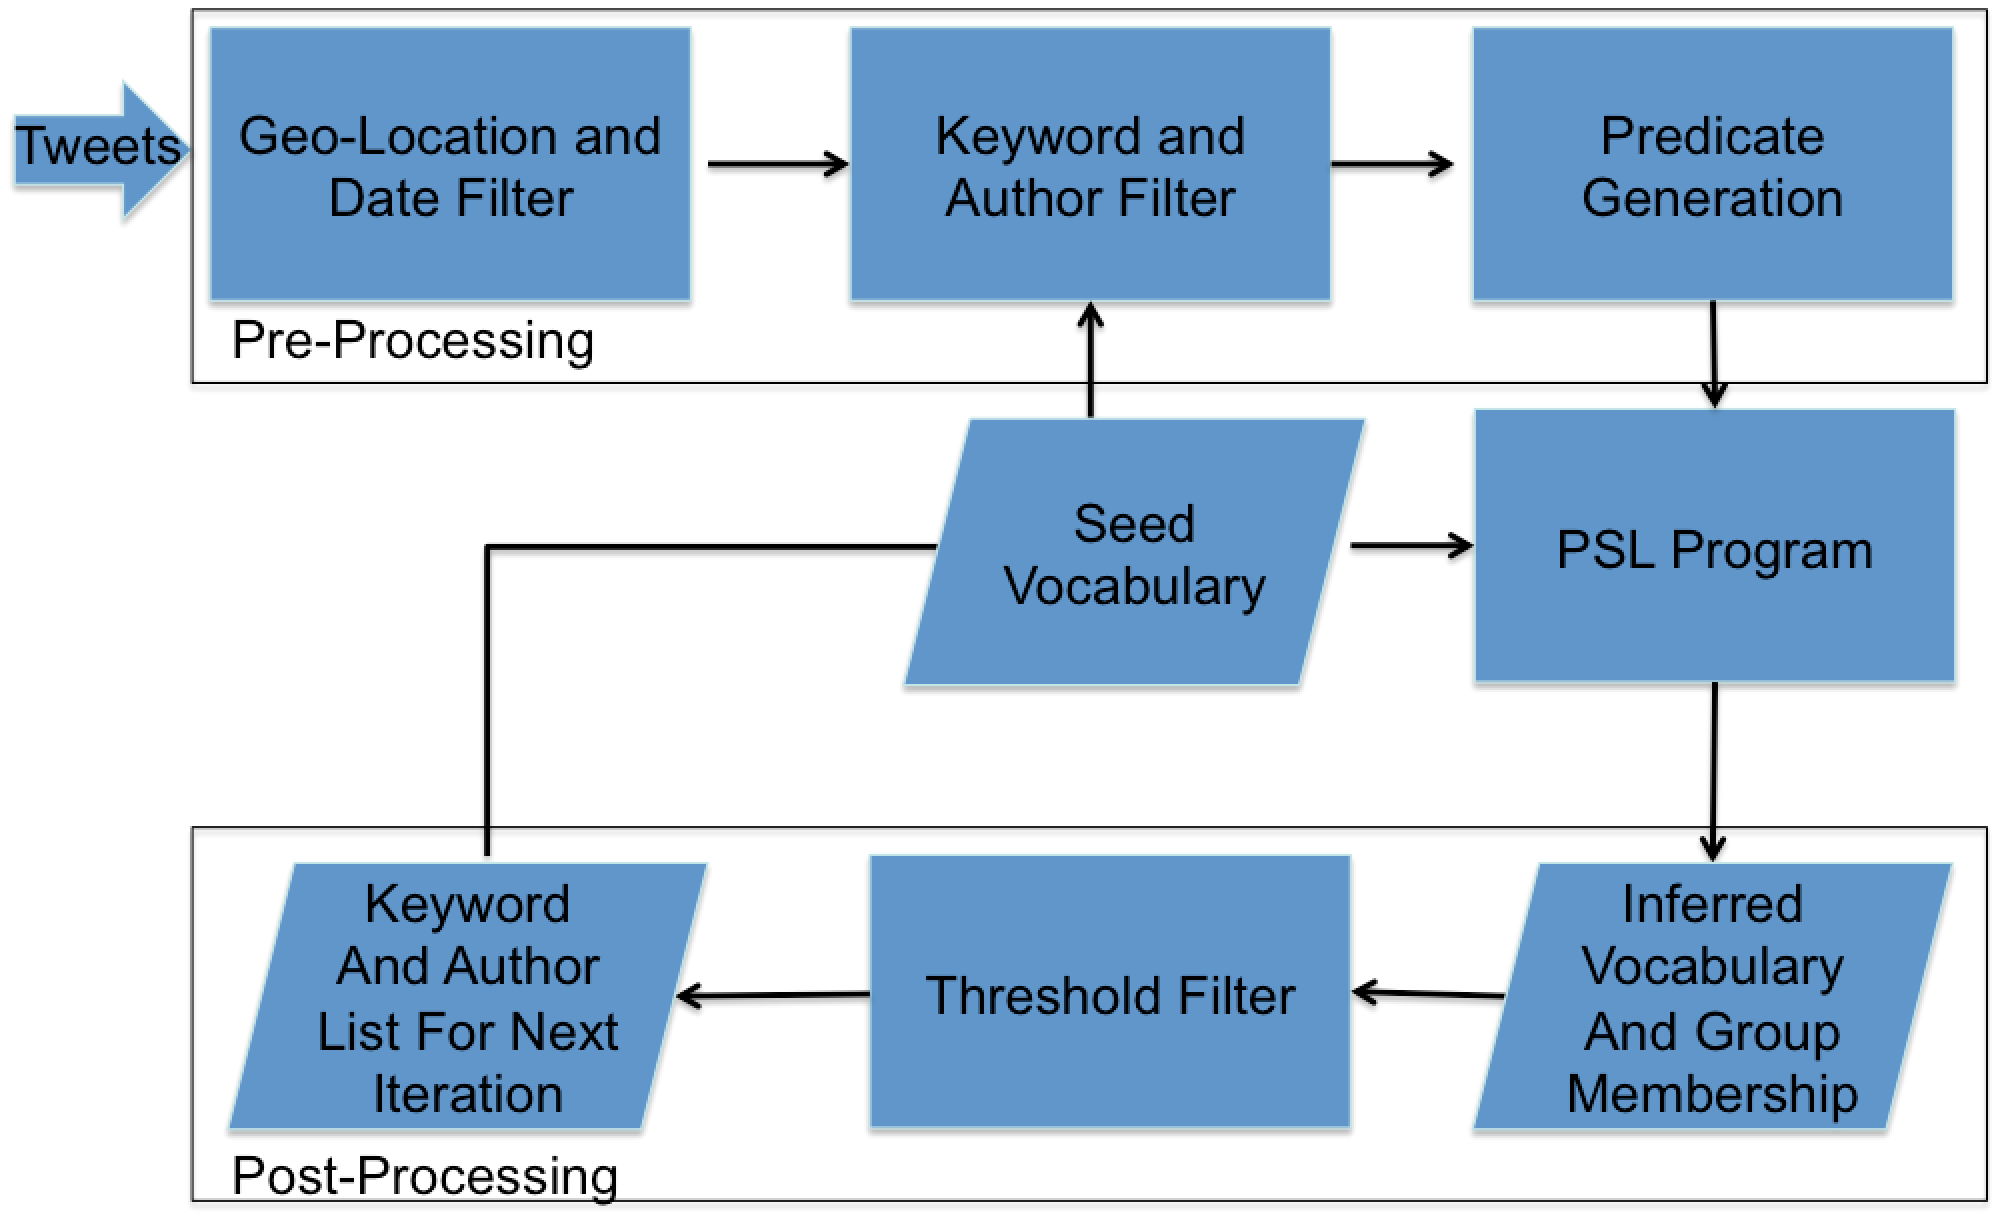
\includegraphics[scale=0.25]{support_files/flowChart.png}
	%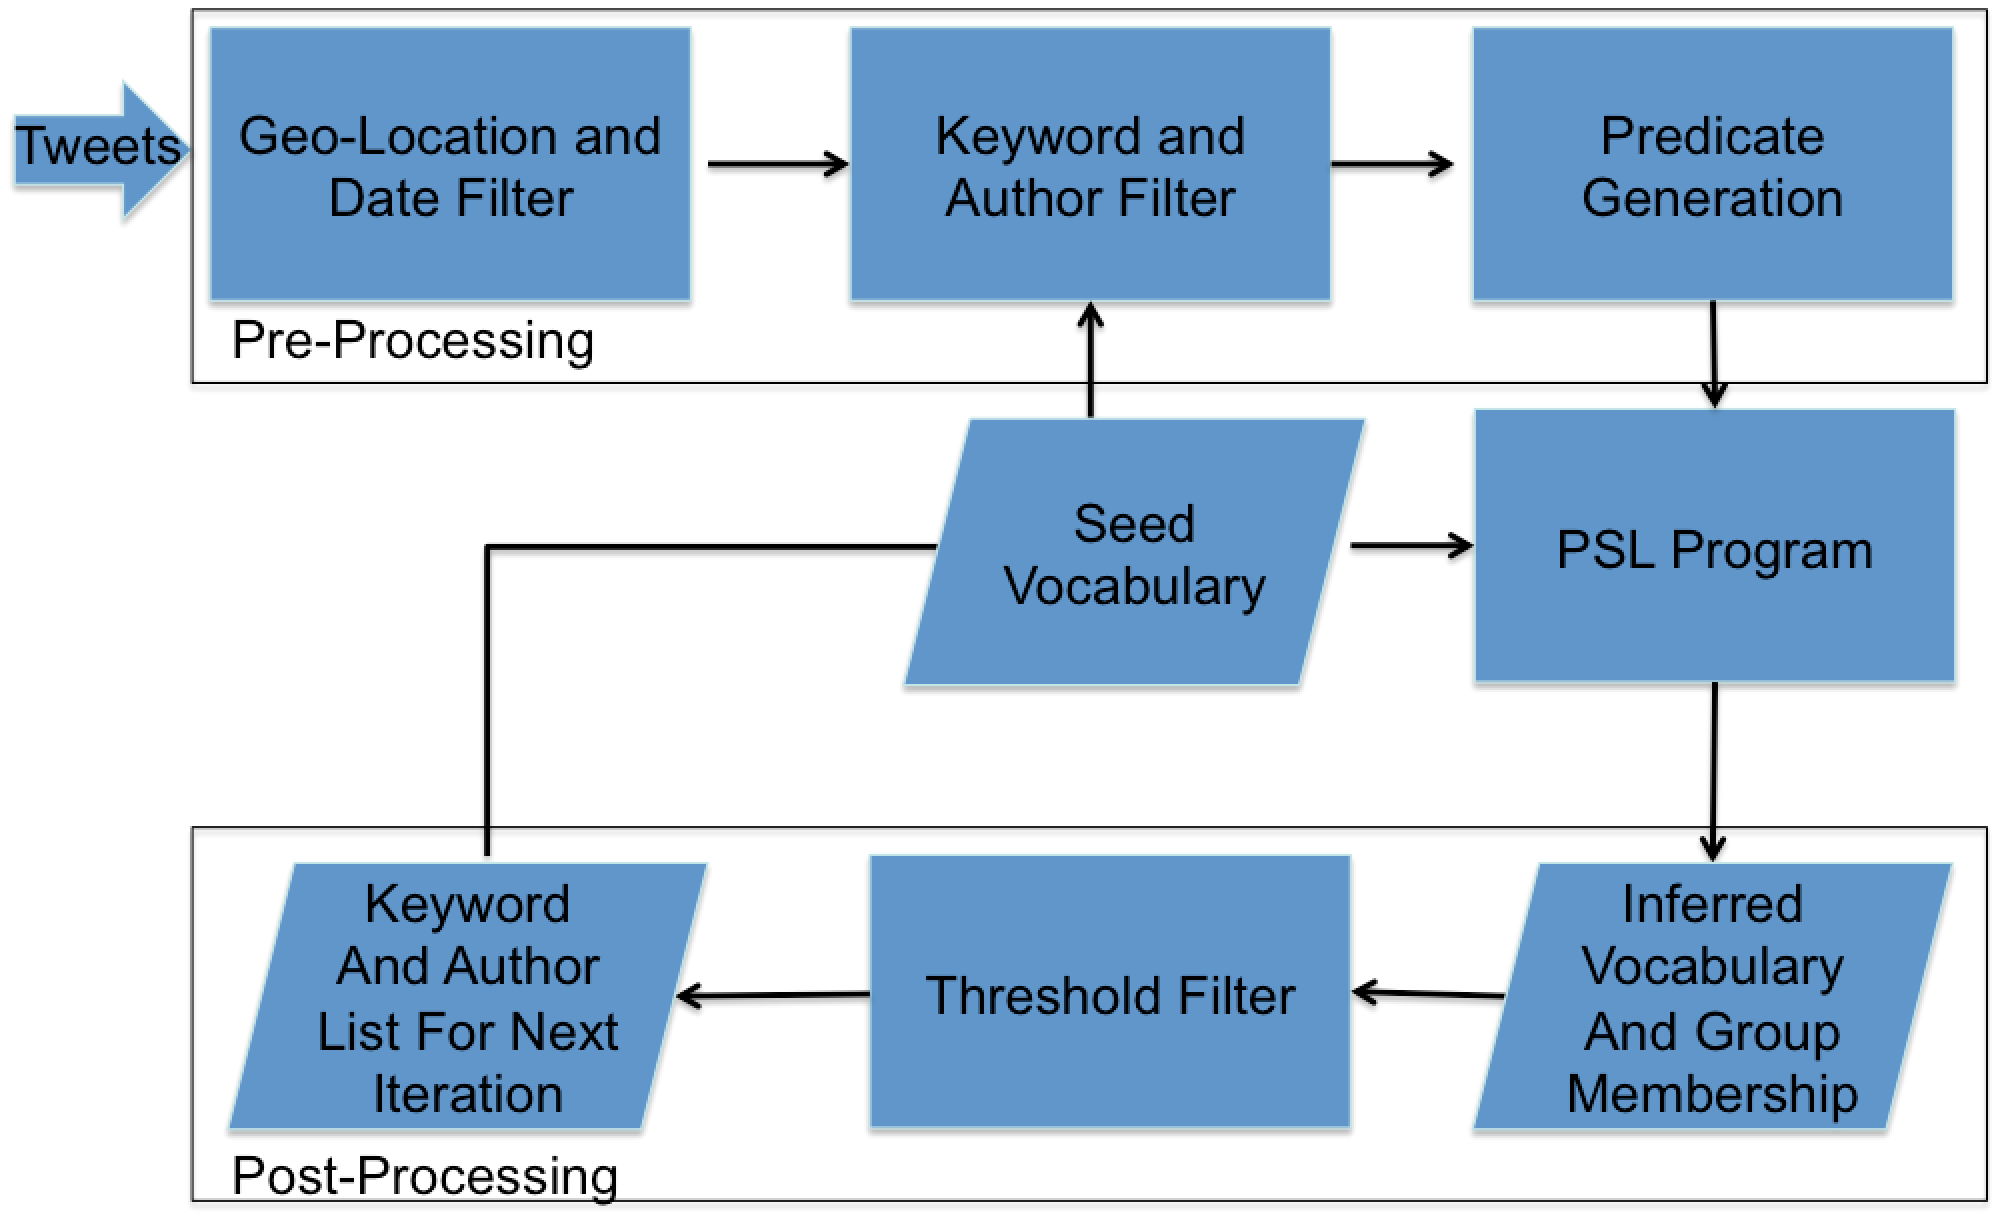
\includegraphics[height=0.25\textheight, width=0.80\textwidth]{support_files/flowChart.png}
	\caption{Design of the query expansion pipeline.}
	\label{fig:flowchart}
\end{figure*}
\section{Probabilistic Soft Logic}
\emph{Probabilistic soft logic} ~\cite{kimmig2012short,broecheler2010probabilistic} is a framework for collective probabilistic reasoning in relational domains.
PSL models have been developed for various problem areas, including opinion diffusion ~\cite{bach2012scaling}, ontology alignment ~\cite{broecheler2010probabilistic}, trust in social networks ~\cite{huang2013flexible}, and knowledge graph identification ~\cite{pujara2013knowledge}.
PSL uses a syntax based on first-order logic to encode probabilistic models, which are declaratively defined as sets of weighted rules and constraints. PSL uses a continuous relaxation of logical truth to interpret these rules as a joint, continuous probability distribution over the truth values of logical atoms. The continuous relaxation enables fast algorithms to perform inference in highly structured models, as well as transparent incorporation of continuous variables and features. Like other rule-based systems, the ability to define complex models using a natural logical syntax streamlines the design process.

In PSL, user-defined \emph{predicates} are used to encode the relationships and attributes, and \emph{rules} capture the dependencies and constraints.
Each rule's antecedent is a conjunction of atoms and its consequent is a disjunction. 
The rules are assigned non-negative weights, which correspond to the likelihood of the rules' satisfaction. 
The set of predicates and weighted rules thus make up a PSL program where known truth values of ground atoms are set from observed data and unknown truth values for the remaining atoms are inferred by finding a maximizing state of a probability distribution defined by the rules.

Given a set of atoms 
$\ell = \{\ell_1,\ldots,\ell_n\}$,
an interpretation defined as 
$I : \ell \rightarrow [0,1]^n$
is a mapping from atoms to soft truth values.
PSL defines a probability distribution over all such interpretations where those that satisfy more ground rules are more probable.
The continuous interpretation of rule satisfaction uses the \emph{Lukasiewicz t-norm} and its corresponding co-norm to define relaxations of the logical AND and OR respectively.
Given interpretation $\mathit{I}$, these relaxations for the logical conjunction ($\wedge$), disjunction ($\vee$), and negation ($\neg$) are as follows:
\begin{align*}
\ell_1 \softand \ell_2 &= \max\{0, I(\ell_1) + I(\ell_2) - 1\},\\
\ell_1 \softor \ell_2 &= \min\{I(\ell_1) + I(\ell_2), 1\},\\
\softneg l_1 &= 1 - I(\ell_1),
\end{align*}  
where we use the tilde modifier (\textasciitilde) to indicate the relaxation of the Boolean domain.
Using the logical algebra and the relaxations above, 
an implication rule $\mathit{r} \equiv \mathit{r_{body}} \rightarrow \mathit{r_{head}} $ is satisfied if and only if the truth value of its head is at least that of its body. The rule's \emph{distance to satisfaction} measures the degree to which this condition is violated.
\begin{center} 
 $\mathit{d_r}(\mathit{I}) =$ max\{0,$\mathit{I(r_{body}} - \mathit{I(r_{head})}$\}
 \end{center}
PSL induces a probability distribution over possible interpretations $\mathit{I}$ over the given set of ground atoms $\mathit{l} $ in the domain. 
Let $\mathit{R}$ be the set of all ground rules that are instances of a rule from the PSL program.  
The probability density function $\mathit{f}$ over $\mathit{I}$ is defined as
\begin{equation}
\label{eq:contimn1}
    f (I) = \frac{1}{Z} \text{exp}[-\sum_{r\in R} \lambda_r (d_r(I))^p]
\end{equation}
\begin{equation}
\label{eq:contimn2}
	Z = \int_{I} \text{exp} [ -\sum_{r\in R} \lambda_r (d_r(I))^p ]
\end{equation}
where~$\lambda_r$ is the weight of the rule~$r$, $Z$ is a normalization constant, and ~$p \in \{1, 2\}$ provides a choice between two different loss functions, linear and quadratic.
The values of the atoms can be further restricted by providing linear equality and inequality constraints, allowing one to encode functional constraints from the domain.

Given a partial interpretation with grounded atoms based on observed evidence, \emph{most probable explanation} (MPE) inference seeks the truth values for the unobserved atoms satisfying the most likely interpretation. 
%Because energy function is convex, MPE inference is solved using a convex optimization. Because of the structure of the energy function constructed from rules, a fast decomposition algorithm is particularly effective for solving this inference optimization
The MPE inference is a convex optimization problem because the energy function is convex. 
This inference optimization can be efficiently solved using a fast decomposition algorithm ~\cite{bach2012scaling,bach2013hinge} by exploiting the structure of the energy function constructed from rules.
\section{Dynamic Query Expansion using PSL}
We use PSL to develop a dynamic query expansion strategy wherein we begin with an
initial set of hashtags or terms (\emph{seed words})
that we believe are indicative of the affinity of a
particular user to a candidate contesting in the election (e.g., these terms are names,
party symbols of the candidate).
We iteratively use PSL inference over successive time windows such that the inference 
from window $w_t$ is used as a prior to window $w_{t+1}$, and the inference from 
that is used for window $w_{t+2}$, and so on.
Figure~\ref{fig:flowchart} illustrates the design of the iterative algorithm for dynamic query expansion.

The initial pre-processing begins with the tweet input stream, which is filtered by a
date range specified by the window size. 
For each election, tweets from a month leading up to the election were used.
After extensive analysis we determined that the optimal window size was three days;
smaller window sizes resulted in not enough data points for probabilistic inference, and
larger window sizes lead to combinatorial explosion as PSL generates rules by
substituting all possible groundings.
Though the optimal window size could vary for different elections depending upon the number of tweets originating from the involved country, we use three days as window size for all elections 
for consistency. 
The tweets passing the date filter are then geocoded using a geolocation algorithm that infers 
the location of a tweet and enables us to localize the set of tweets analyzed.
The geolocation algorithm tags the tweets with a location using the
GPS coordinates of the tweet, if available, or landmarks and locations mentioned in the tweet 
or in the author's profile. 
For tweets that do not have any of these, we use 
a label propagation algorithm to infer the author's location through his/her network.

The geotagged tweets are then tracked for the presence of a hashtag from 
the vocabulary for that particular iteration.
In addition to filtering tweets using the vocabulary the authors whose affiliations are already inferred by the system are also used as a filtering criteria.
The information from
the tweets are then coded into PSL predicates and fed into the inference process.
The PSL program infers the hashtags and tweeters that are mostly associated with 
a particular candidate. 
Each author and hashtag's association with a candidate is measured using the truth value 
of the predicate grounding.
In the post-processing step, these truth values are filtered by a threshold value to identify the hashtags and authors strongly associated to a candidate.
These hashtags become a part of the vocabulary of the candidate and along with the users identified are used as a filter criterion for the next iteration.
This iterative process proceeds until the day before the election when we obtain the final vocabulary which are strongly associated with a candidate.

Within the PSL program we define predicates to encode the network. 
The predicates $\textsc{Tweeted}(U,T)$ and $\textsc{Contains}(T,W)$  capture the fact that a user $U$ tweeted a tweet $T$ and tweet $T$ contains hashtag $W$ respectively. 
Similarly, the belief that an user $U$ or hashtag $W$ is affiliated/associated to the group $G$ is encoded as $\textsc{IsMember}(U,G)$ and $\textsc{Belongs}(W,G)$ respectively.
In order to capture the temporal connectivity between the iterations, in addition to the initiating the inference process with the rule
\begin{align*}
\textsc{SeedWord}(W,G) \Rightarrow \textsc{Belongs}(W,G)
\end{align*}
we define additional rules such as
\begin{align*}
\textsc{WasMember}(A,G) \Rightarrow \textsc{IsMember}(A,G)
\end{align*}
\begin{align*}
\textsc{Belonged}(W,G) \Rightarrow \textsc{Belongs}(W,G)
\end{align*}
where the predicates $\textsc{WasMember}$ and $\textsc{Belonged}$ are inferences from the previous time window and are loaded in as  priors for the current iteration.
These rules are weighted slightly lower than the recursive rules below so that the system overcomes the bias it had learned in light of new, more convincing evidence.
This way hashtags that are more indicative of a user's affiliation are assigned stronger truth values or weights for every successive iteration and the truth values of hashtags that are not are reduced.
The same reasoning applies to the user-candidate affiliations (memberships).
Below we outline the recursive PSL rules that grows the hashtag preferences and the user affiliations. 
\begin{align*}
\begin{split}
\textsc{Tweeted}(A,T) 
	\softand \textsc{Contains}(T,W)
	\softand \textsc{Belongs}(W,G) \\ 
	\softand \textsc{Positive}(T)
	\Rightarrow \textsc{IsMember}(A,G)
\end{split}
\end{align*}

\begin{align*}
\begin{split}
\textsc{Tweeted}(A,T)
	 \softand \textsc{Contains}(T,W)
	\softand \textsc{Belongs}(W,G)\\
	 \softand \textsc{Negative}(T)
	\Rightarrow \sim \textsc{IsMember}(A,G)
\end{split}
\end{align*}

\begin{align*}
\begin{split}
\textsc{IsMember}(A,G)
	 \softand \textsc{Tweeted}(A,T)
	\softand \textsc{Contains}(T,W)\\
	 \softand \textsc{Positive}(T) 
	\Rightarrow \textsc{Belongs}(W,G)
\end{split}
\end{align*}

\begin{align*}
\begin{split}
\textsc{IsMember}(A,G) 
	\softand \textsc{Tweeted}(A,T)
	\softand \textsc{Contains}(T,W)\\
	\softand \textsc{Negative}(T)
	\Rightarrow \sim \textsc{Belongs}(W,G)
\end{split}
\end{align*}
Here $\textsc{Positive}$ and $\textsc{Negative}$ are predicates whose truth values are calculated from the sentiment of the tweet such that the highly positive tweets get a truth value closer to $1.0$ for the predicate $\textsc{Positive}$ and highly negative tweets are assigned a truth value of $1.0$ for the predicate $\textsc{Negative}$. 
Since PSL works under the closed world assumption, we do not need to specify the groundings that are false i.e., positive tweets are not assigned $0.0$ for the predicate $\textsc{Negative}$ and vice-versa.
For tweets that do not have a positive or negative orientation we assign a truth value of $0.5$ for both the $\textsc{Positive}$ and $\textsc{Negative}$ predicates.
\begin{figure*}
	\centering
	\subfloat[Day 0]
	{
		
\includegraphics[width=0.5\textwidth, height=0.17\textheight]{support_files/caprilesWordCloud1.png}
		\label{fig:wordCloud1}
	} 
	\subfloat[Day 6]
	{
		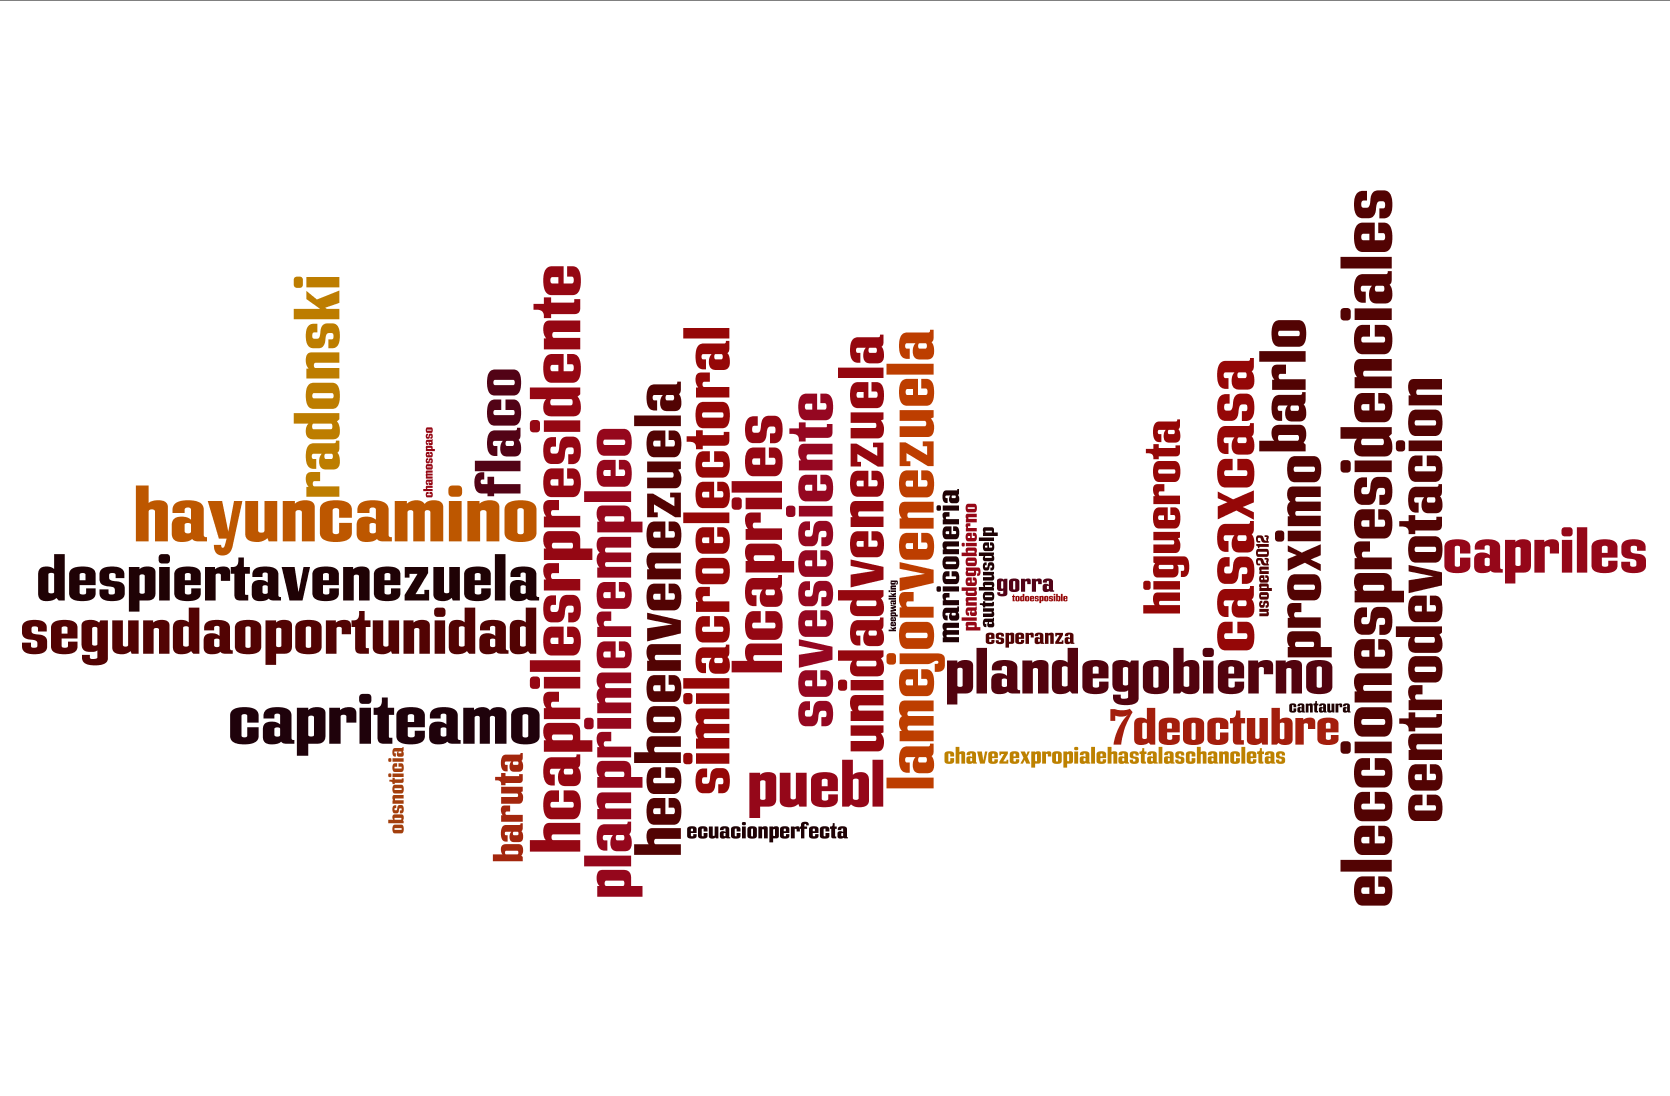
\includegraphics[width=0.5\textwidth, height=0.17\textheight]{support_files/caprilesWordCloud2.png}
		\label{fig:wordCloud2}
	} \\
	\noindent 
	\subfloat[Day 15]
	{
		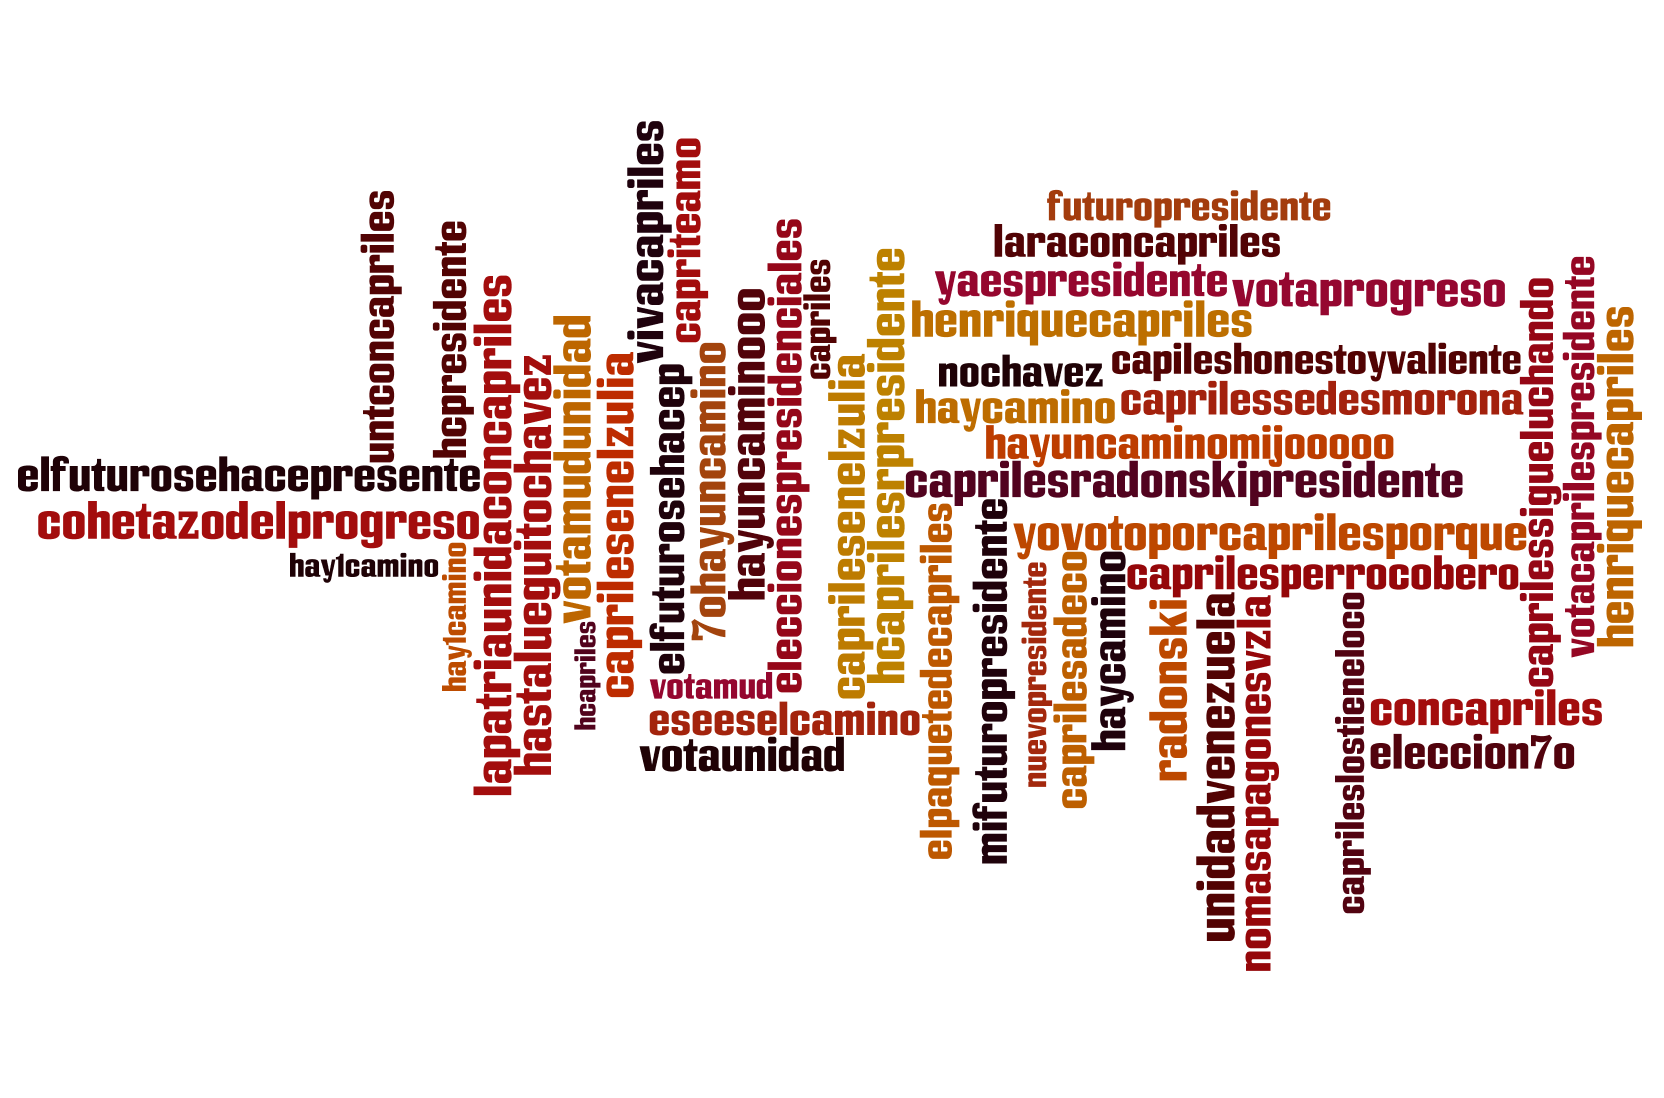
\includegraphics[width=0.5\textwidth, height=0.17\textheight]{support_files/caprilesWordCloud3.png}
		\label{fig:wordCloud3}
	}
	\subfloat[Day 30]
	{
		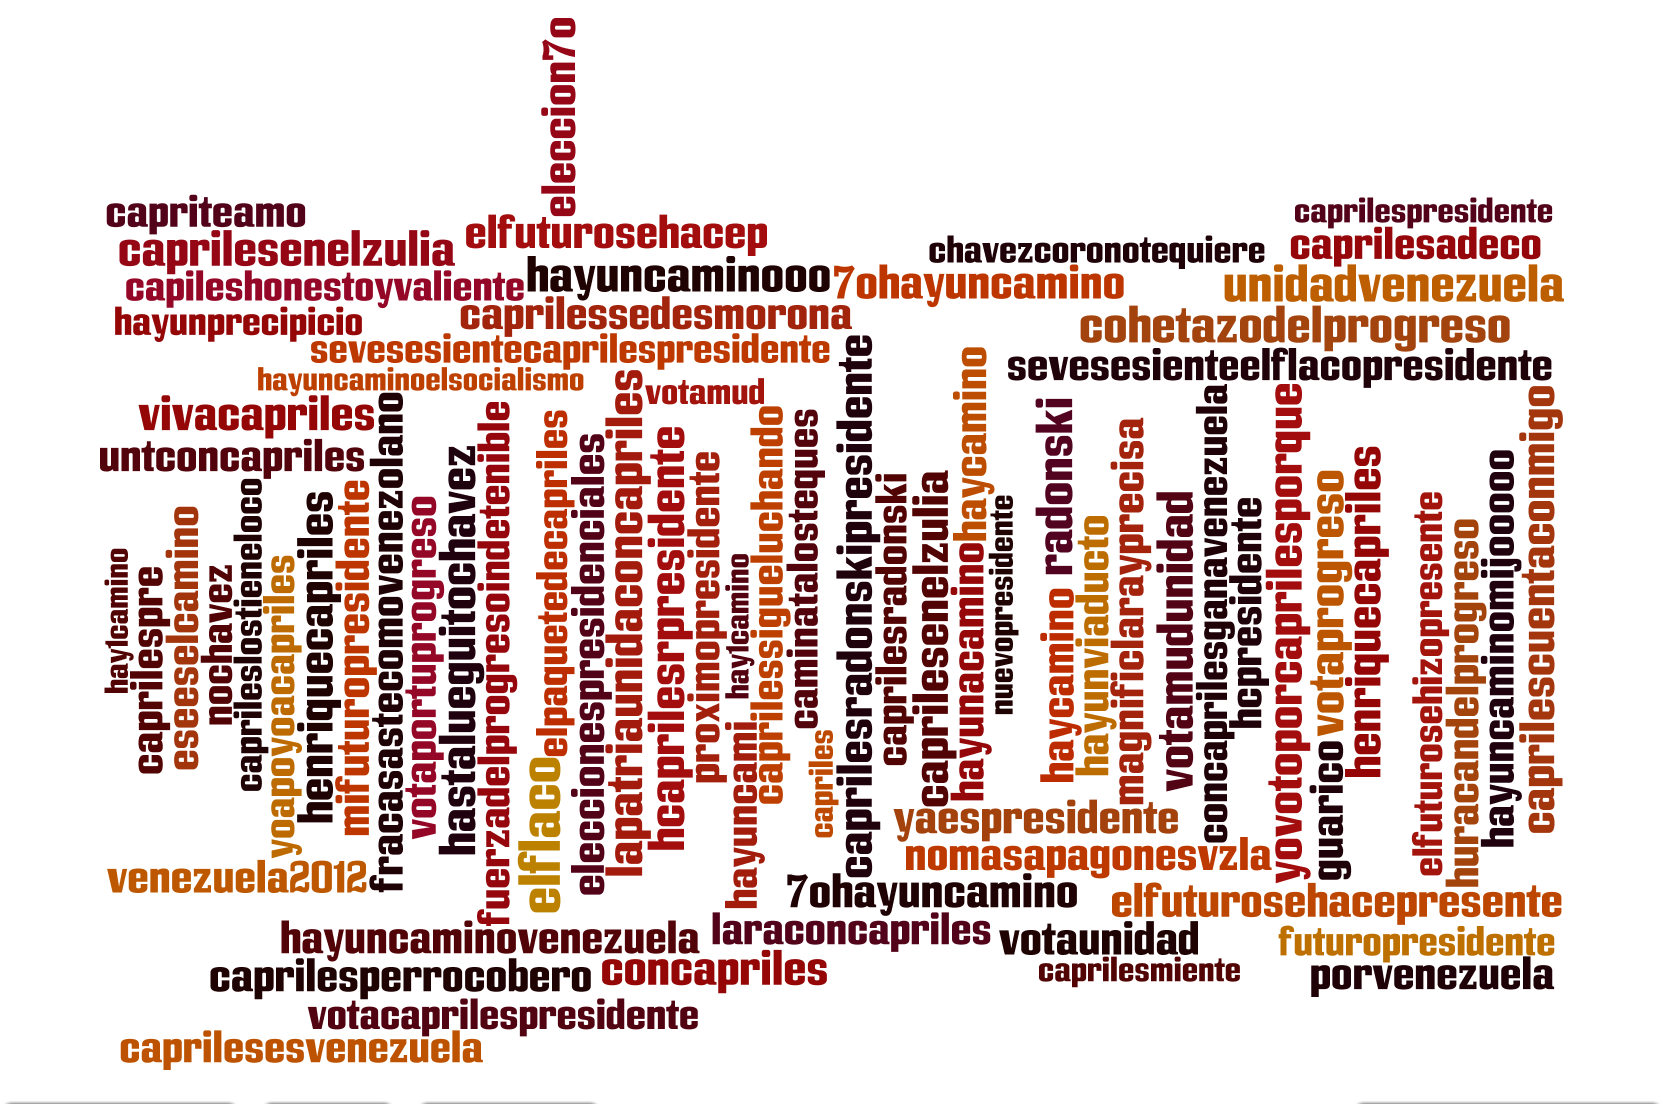
\includegraphics[width=0.5\textwidth, height=0.17\textheight]{support_files/caprilesWordCloud4.png}
		\label{fig:wordCloud4}
	}
	\caption{Evolution of hashtags for Henrique Capriles} 
	\label{fig:wordCloud}
\end{figure*}

We also defined rules that encode how ideologies propagate in a social media, specifically Twitter.
For example, the first rule below states if one author retweets a tweet created by another author then it can be assumed that the former is endorsing the opinion of the latter and hence likely to have the same political affiliation. 
Similarly a person mentioning another person in a positive connotation is assumed to share similar views.
The rules below detail the propagation of affiliation based on social interactions.
\begin{align*}
\begin{split}
\textsc{IsMember}(B,G) 
	\softand \textsc{Tweeted}(A,T)
	\softand \textsc{ReTweet}(T,B)\\
	\Rightarrow \textsc{IsMember}(A,G)
\end{split}
\end{align*}
\begin{align*}
\begin{split}
\textsc{IsMember}(B,G) 
	\softand \textsc{Tweeted}(A,T)
	\softand \textsc{Mentions}(T,B)\\
	\softand \textsc{Positive}(T)
	\Rightarrow \textsc{IsMember}(A,G)
\end{split}
\end{align*}
\begin{align*}
\begin{split}
\textsc{IsMember}(B,G) 
	\softand \textsc{Tweeted}(A,T)
	\softand \textsc{Mentions}(T,B)\\
	\softand \textsc{Negative}(T)
	\Rightarrow \sim \textsc{IsMember}(A,G)
\end{split}
\end{align*}
The last two rules defined below encode the assumption that when two hashtags co-occur and one is a name of a candidate then the other hashtag is bound to be about the candidate too.
Since these two rules have two variables $\textsc{W1}$ and $\textsc{W2}$, the number for rules generated by substituting actual groundings (hashtags) increase rapidly with the number of tweets feeding into the inference process. 
This was a major contributing factor to the memory issues detailed in the optimal window size discussion.
\begin{align*}
\begin{split}
\textsc{Contains}(T,W1)
 \softand \textsc{Contains}(T,W2)
  \softand \\
   \textsc{SeedWord}(W1,G)
  \softand \textsc{Positive}(T) \\
	\Rightarrow \textsc{Belongs}(W2,G)
\end{split}
\end{align*}

\begin{align*}
\begin{split}
\textsc{Contains}(T,W1) 
	\softand \textsc{Contains}(T,W2)
	\softand \\
	 \textsc{SeedWord}(W1,G)
	\softand \textsc{Negative}(T)\\
	\Rightarrow \sim \textsc{Belongs}(W2,G)
\end{split}
\end{align*}
In addition to the rules, we also define constraints on the $\textsc{Belongs}$ and $\textsc{IsMember}$ predicates so that a particular hashtag or author can be associated to at most one candidate. 
Once all the tweets are loaded into the PSL program as predicates, we start the inference process by closing all the predicates except $\textsc{IsMember}$ and $\textsc{Belongs}$. 
This way, only the truth values of these two predicates are inferred and the other groundings of the closed predicates are regarded as facts.

\section{Experimental Results}
Our experimental results are organized alongside the following questions:
\begin{itemize}
\item How adept is our PSL-based dynamic query expansion algorithm at extracting relevant hashtags/keywords over the course
of an election season?
\item How does the performance of forecasting algorithms improve using our expanded vocabularies?
\end{itemize}
We answer each of these questions next.

\subsection{Election vocabularies inferred}

\noindent
{\bf Venezuela:} %Figure~\ref{fig:wordgrowth} shows  how the vocabulary grows with each iteration for the two candidates who contested the Venezuelan presidential election on October 7th 2012.
Figure~\ref{fig:wordCloud} shows how the hashtags for Henrique Capriles evolved during the month leading up to the election.
Initially in Figure~\ref{fig:wordCloud1} the system begins with only a few hand picked hashtags that constitute the seed vocabulary. 
After a few iterations Figure~\ref{fig:wordCloud2} shows how the vocabulary has grown.
However, not all the words identified until now remain in the final vocabulary as the system drops certain words in successive iterations.
At the same time it is also noticed that hashtags like ``capriles" and ``hayuncamino" which are very strongly associated with Capriles consistently remain as the top ranked hashtags even after ten iterations (Figure~\ref{fig:wordCloud4}). 
It is also interesting to note that the algorithm identified hashtags like ``nochavez" (Figure\ref{fig:wordCloud3}) and attributed it rightly to Hugo Ch\'{a}vez's primary contender, i.e., Capriles. 
\begin{figure*}[Ht]
	\centering
	%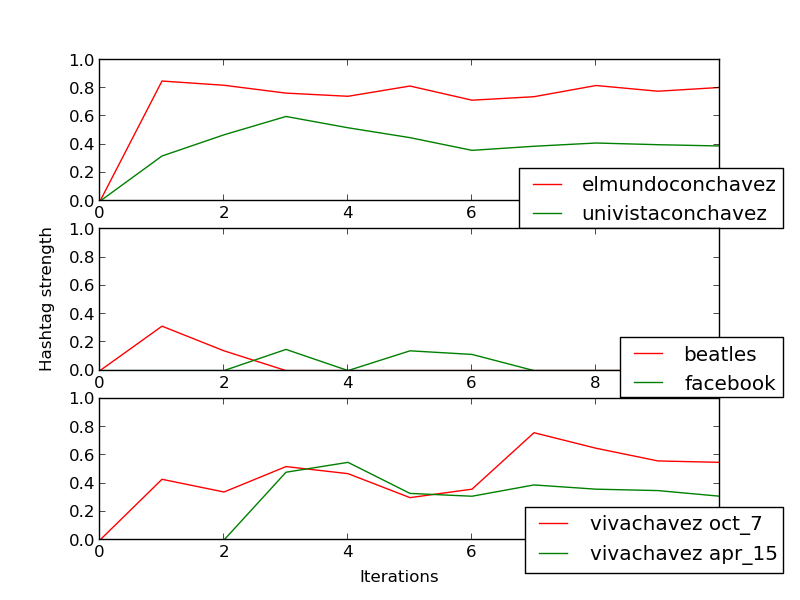
\includegraphics[scale=0.40]{support_files/hashTagTimeSeries.png}\\
	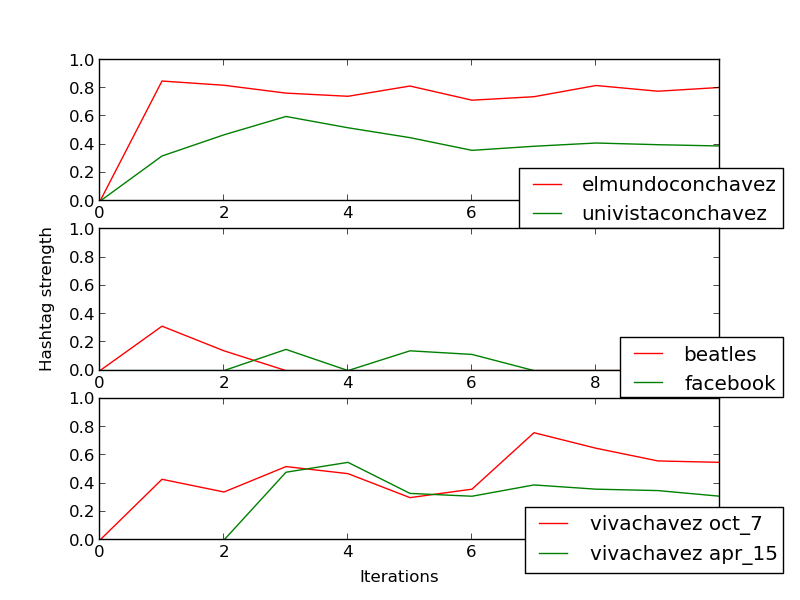
\includegraphics[height=0.25\textheight, width=0.80\textwidth]{support_files/hashTagTimeSeries.png}
	\caption{Time series comparison for different hashtags identified for Hugo Ch\'{a}vez.}
	\label{fig:timeSeries}
\end{figure*}
In Figure~\ref{fig:timeSeries}, the first plot elucidates how hashtags like \emph{``elmnduconchavez"} and 
\emph{``univistaconchavez"} remain highly associated with Hugo Ch\'{a}vez for the October 7th Presidential election. 
These hashtags remain indicative of a user's affiliation throughout the month leading up to the election.
Meanwhile hashtags such as \emph{"beatles"} and \emph{"facebook"} (in second plot) show spikes in their time series primarily because users affiliated with Ch\'{a}vez used them during that time window. 
But as the iterative process continues, the system drops these non-informative words.
The third plot presents another interesting observation.
Hugo Ch\'{a}vez who had won the election on October 7, 2012 was diagnosed with cancer and passed away
before being sworn in as the President.
This triggered a re-election on April 15, 2013 where Nicolas Maduro, who had assumed the role of acting president then, competed 
against Henrique Capriles in the Presidential race.
The hashtag \emph{``vivachavez"} is part of both the elections, despite the 
fact that Hugo Ch\'{a}vez did not compete in the second election.
It is picked up as a phrase commonly used by supporters of Nicholas Maduro whose election campaign was strategized around the death of Hugo Ch\'{a}vez to garner sympathy and mobilize support.
Similarly variations of the hashtags \emph{``hayuncamino"} and \emph{``unidadvenuzela"} were returned 
for Henrique Capriles for both these elections.
The tag MUD is for ``Mesa de la Unidad Democratica” (Democratic Unity Roundtable) that was the organization created for the opposition to Ch\'{a}vez. 
The vocabulary grows to include other terms associated to the campaign, as the official slogan for the opposition ``hayuncamino” (there is a road). 
Others relate to programs that Capriles wanted to implement, such as ``planprimerempleo” (First Job Program). 

\noindent	
{\bf Mexico:} A general election in Mexico took place on July 1st, 2012.
The two front runners where Enrique Pe\'{n}a Nieto (EPN) and Andres Manuel L\'{o}pez Obrador (AMLO).
The tags (Figure~\ref{fig:mexicowordCloud}) show the contest between these two candidates, the first belonging to the “Partido Institucional Revolucionario” (PRI). 
Among the tags we can also find reference to the “yosoy132” student movement that became a key player during the election. 
%We have against AMLO some as “niunvotoalpeje” (no one vote for AMLO) or against EPN “soyantipri” (I am against PRI).
We also see “niunvotoalpeje” (no one vote for AMLO) and “soyantipri” (I am against PRI) which are attributed against AMLO and EPN respectively.

\noindent
{\bf Paraguay:}
Figure~\ref{fig:paraguaywordCloud} details the election between Horacio Cartes from the Partido Colorado and Efrain Alegre from Alianza Paraguay. 
The incumbent president belonged to Partido Colorado and we can see some tags talking about a protest vote: “votocastigoya” (protest vote now). 
Also references from their campaign to each candidate as “yovotoporefrain” (I vote for efrain) or “todosconcartesavanzapais” (everyone with cartes, the country goes forward) are seen.

\noindent
{\bf Honduras:}
In November 2013 Honduras had a general election to choose President, Congress and local officials. 
The wife of former President Zelaya, Xiomara Castro, contended against Juan Orlando Hernandez from the incumbent Partido Nacional. 
Both candidates showed similar numbers in the polls before the election. 
We can find tags that either support Xiomara, like “xiomarapresidenta” (Xiomara President), “hondurastienepresidenta” (Honduras has a female president) or against her, “noaxiomara” (no to Xiomara) in Figure~\ref{fig:honduraswordCloud}.

\noindent
{\bf Ecuador:}
Ecuador had a first round for the presidential election on February 17th, 2013 where Rafael Correa obtained more than 50\% of the votes needed to avoid a second round. 
From the tags(Figure~\ref{fig:ecuadorwordCloud}) we can read support in phrases such as “yatenemospresidente” (we have elected president) or “tenemosarafael” (we have Rafael). 
There are some references to other candidates such as “lassopresidente” (candidate Lasso president).

\begin{figure*}
	\centering
	\subfloat[Nov 24]
	{
		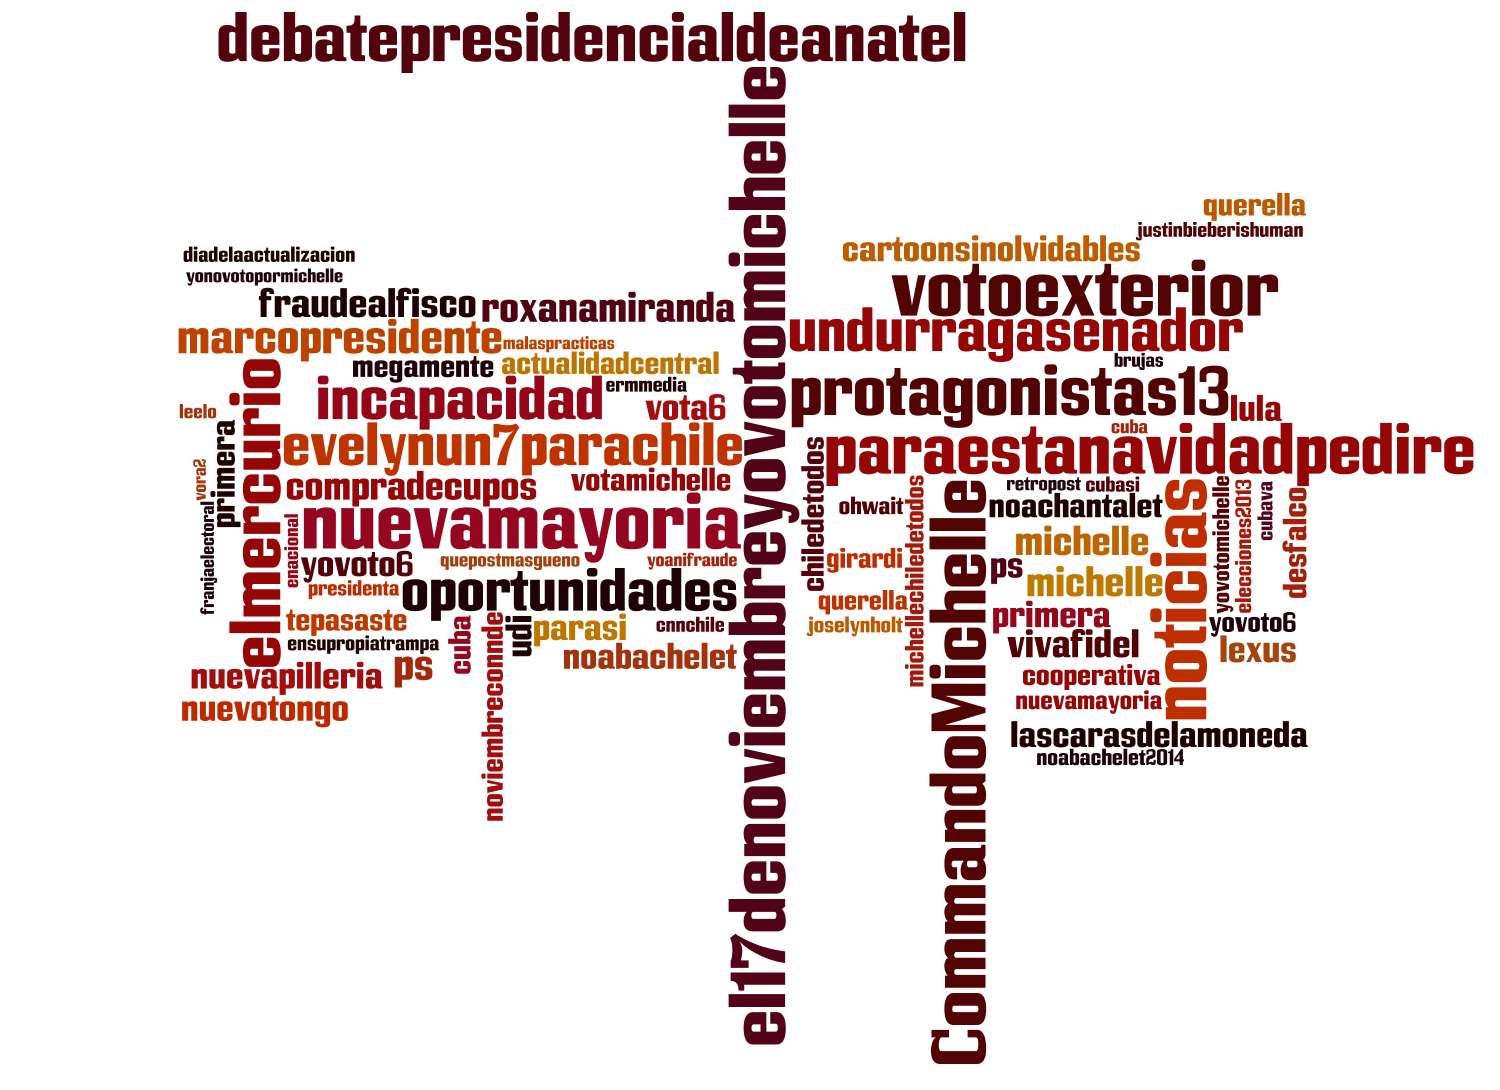
\includegraphics[width=0.5\textwidth, height=0.3\textheight]{support_files/bacheletWordCloud1.png}
		\label{fig:bacheletwordCloud1}
	} 
	\subfloat[Dec 15]
	{
		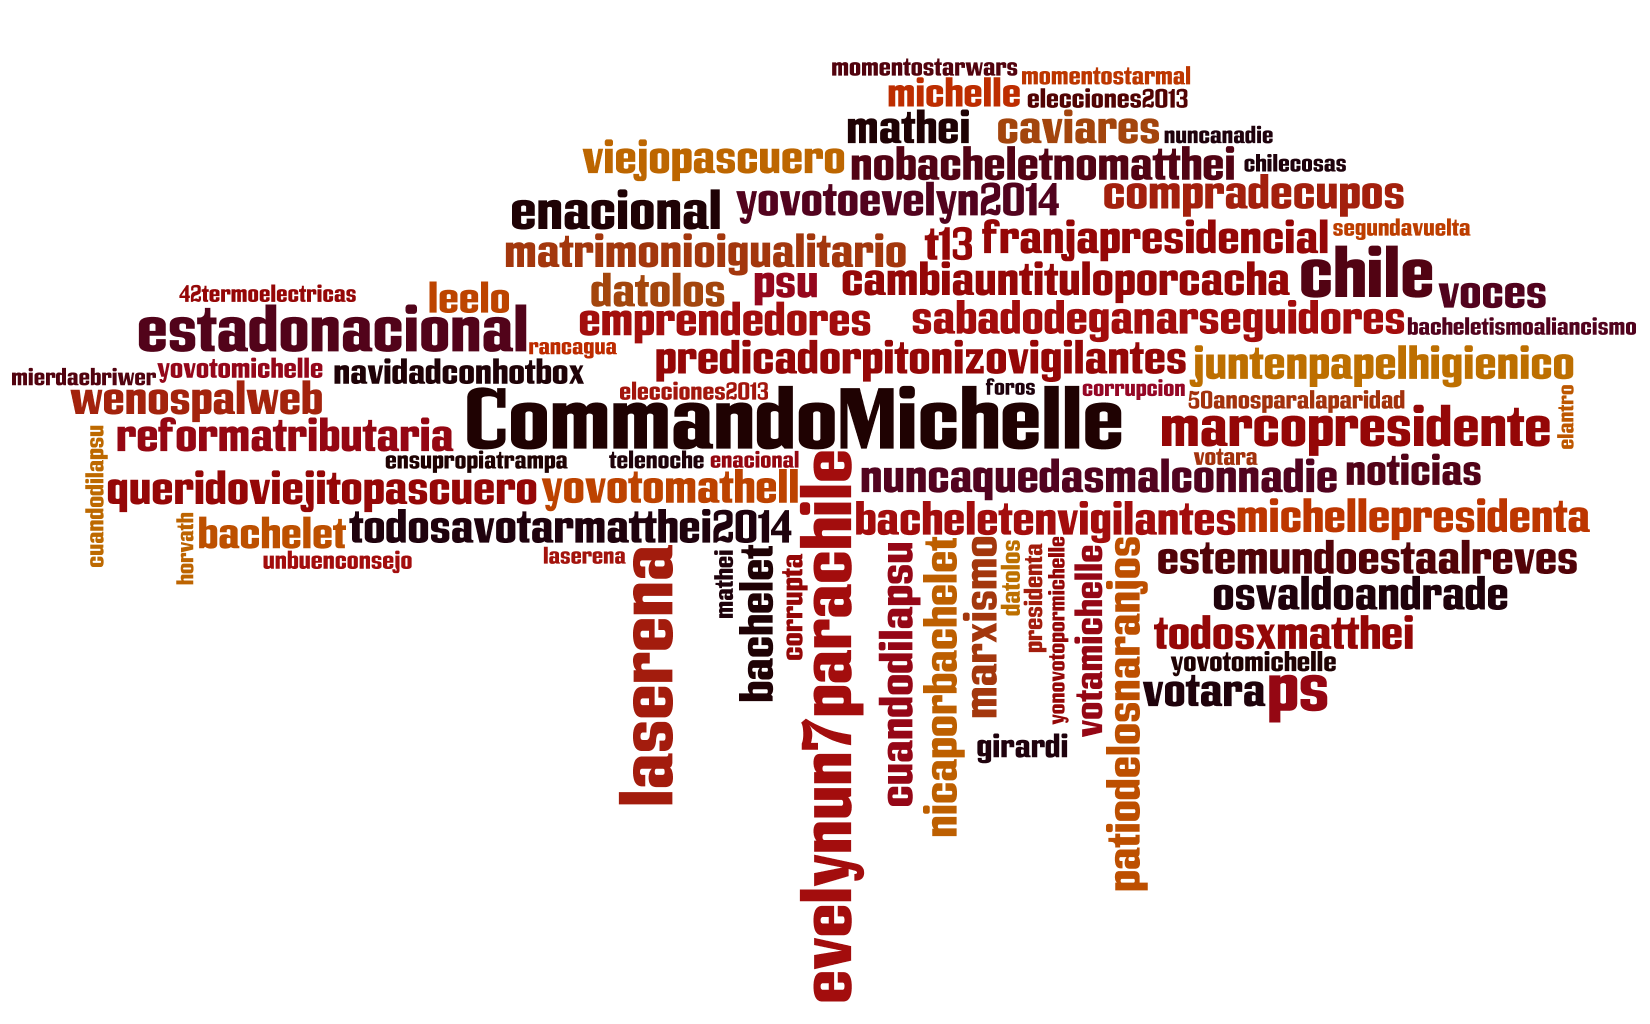
\includegraphics[width=0.5\textwidth, height=0.3\textheight]{support_files/bacheletWordCloud2.png}
		\label{fig:bacheletwordCloud2}
	}
	\caption{Hashtags identified for Michelle Bachelet} 
	\label{fig:bacheletwordCloud}
\end{figure*}
\begin{figure*}
	\centering
	\subfloat[Mexico]
	{
		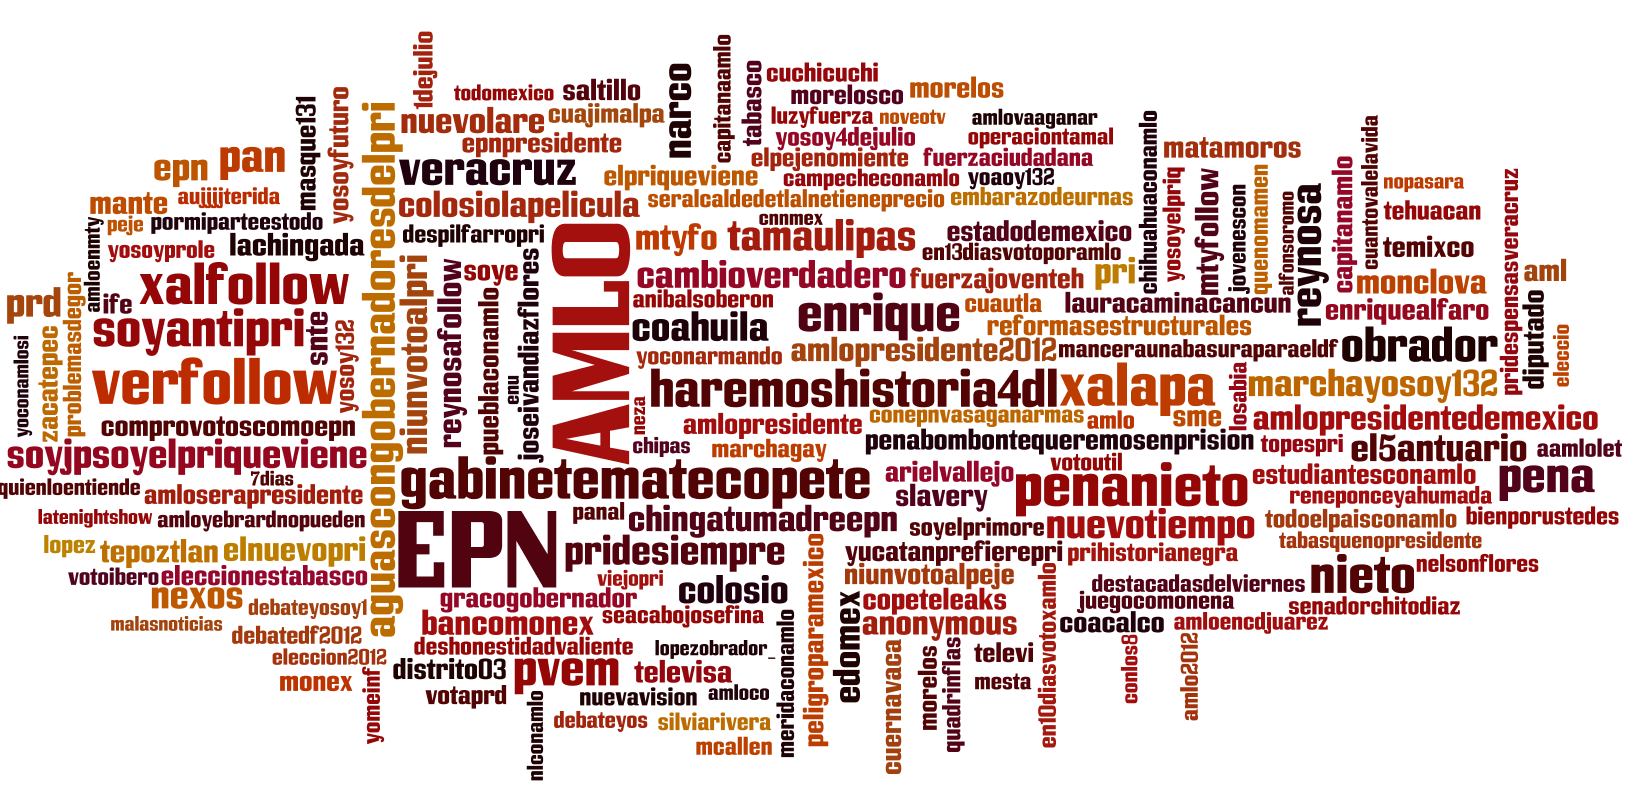
\includegraphics[width=0.5\textwidth, height=0.17\textheight]{support_files/mexicoWordCloud.png}
		\label{fig:mexicowordCloud}
	} 
	\subfloat[Paraguay]
	{
		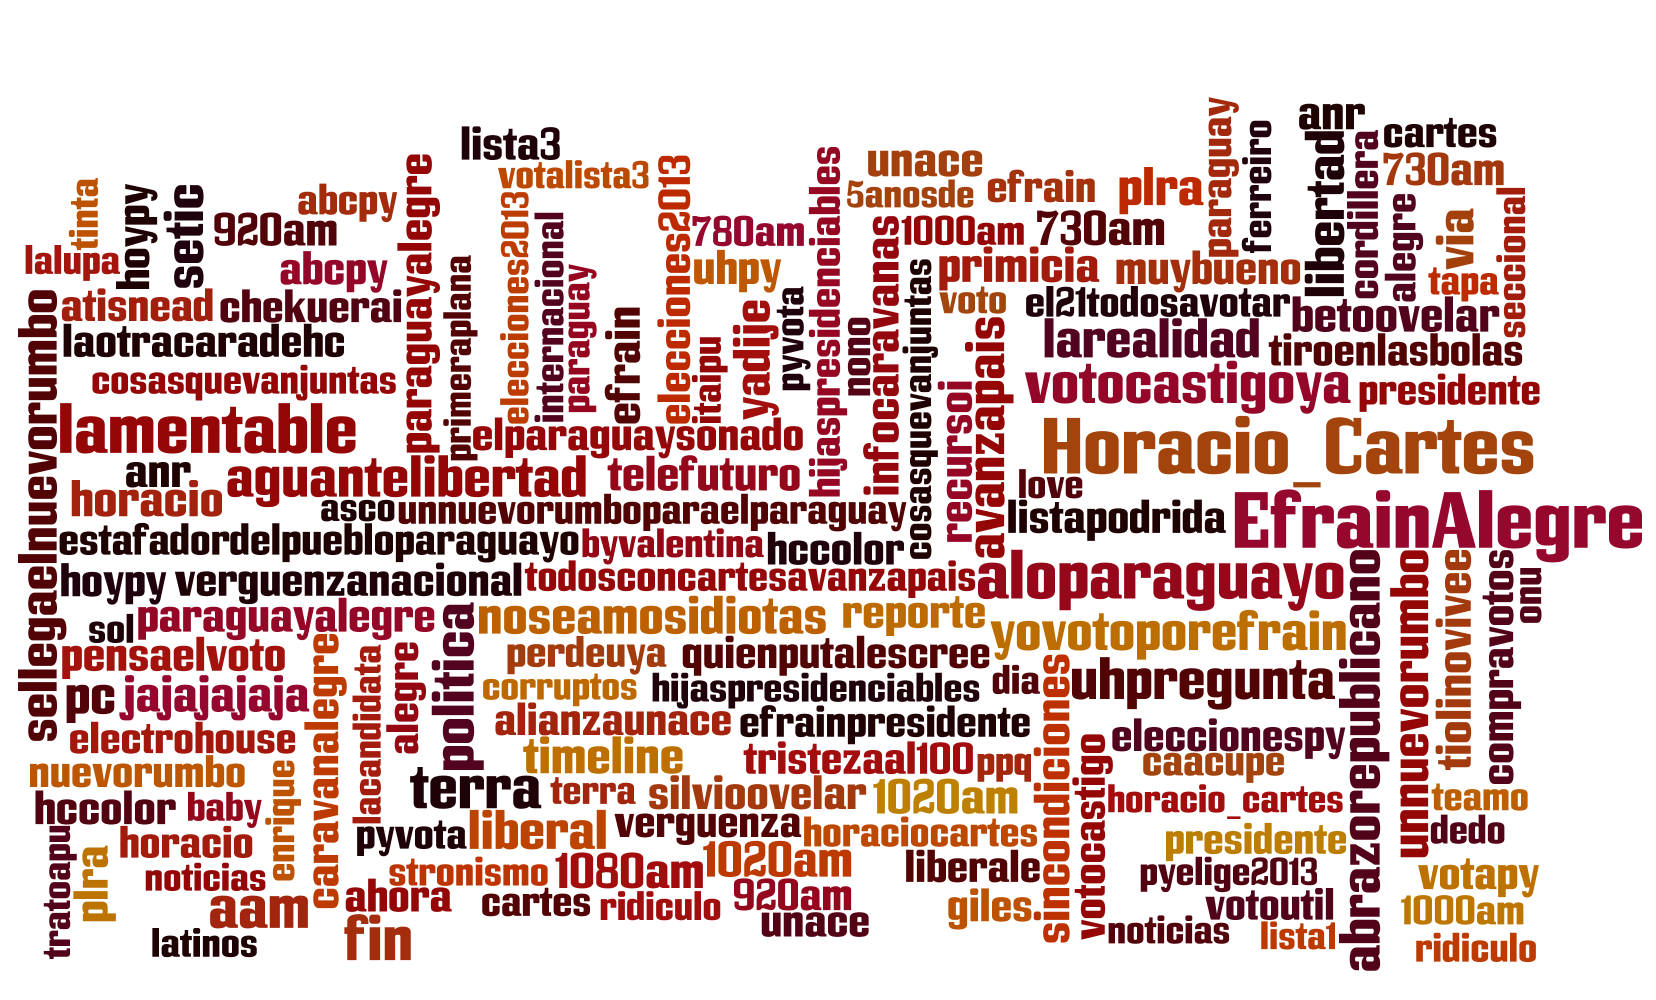
\includegraphics[width=0.5\textwidth, height=0.17\textheight]{support_files/paraguayWordCloud.png}
		\label{fig:paraguaywordCloud}
	} \\
	\noindent 
	\subfloat[Honduras]
	{
		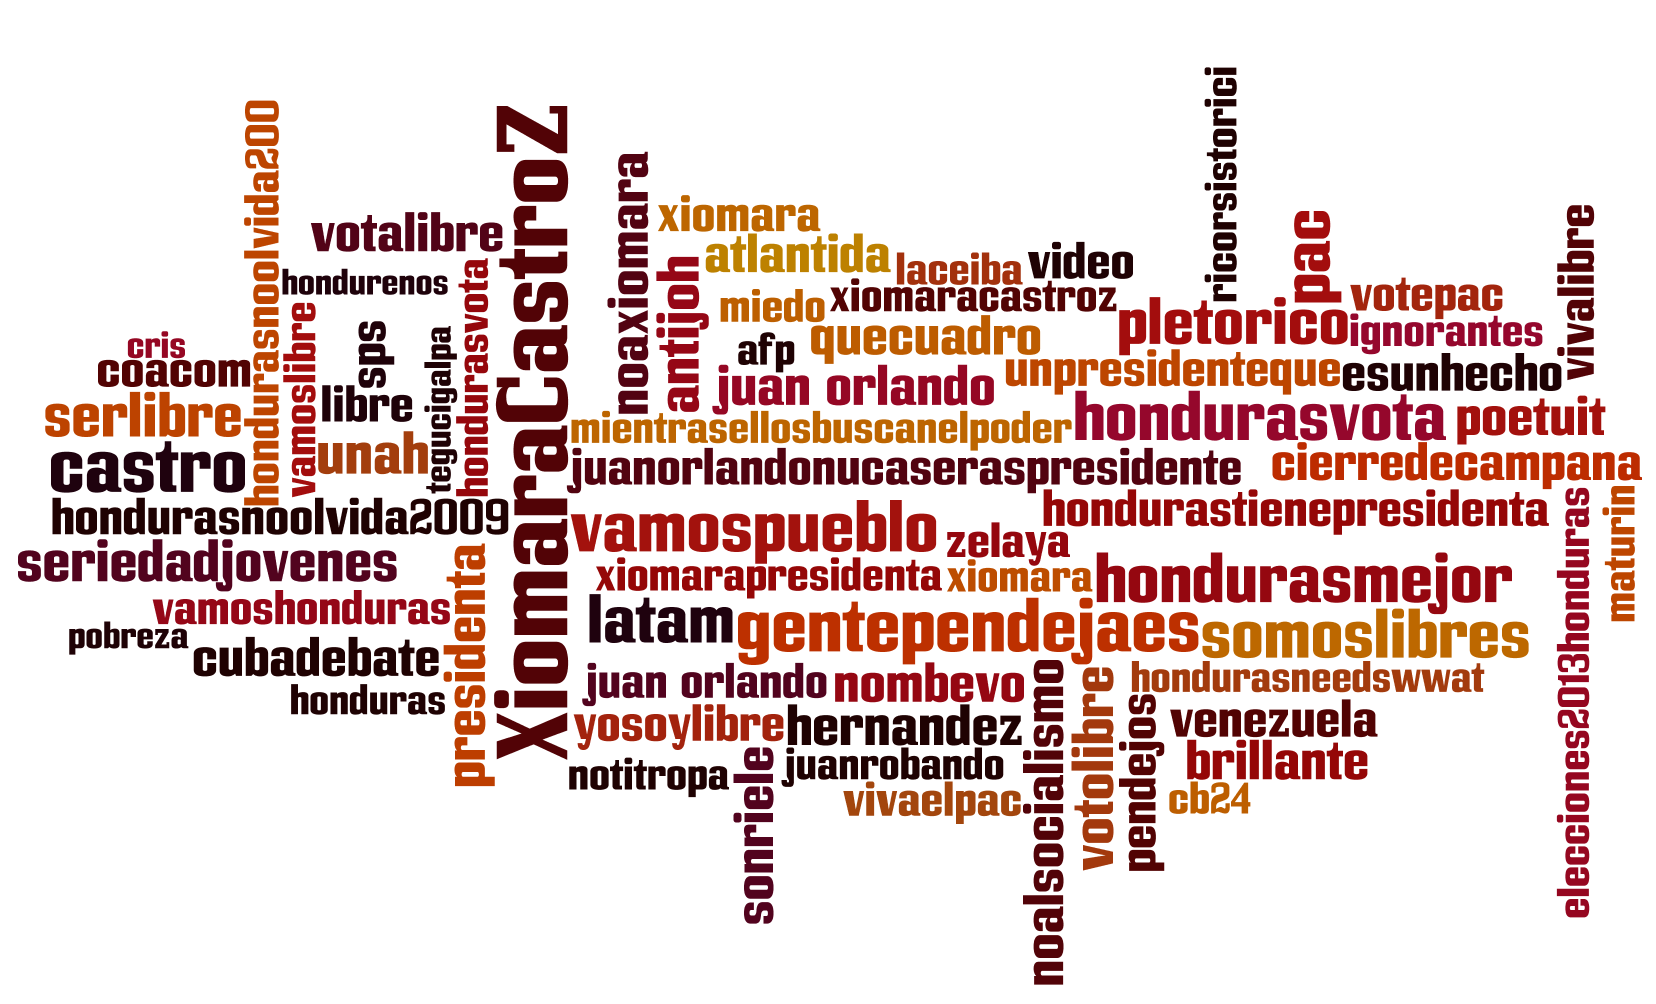
\includegraphics[width=0.5\textwidth, height=0.17\textheight]{support_files/hondurasWordCloud.png}
		\label{fig:honduraswordCloud}
	}
	\subfloat[Ecuador]
	{
		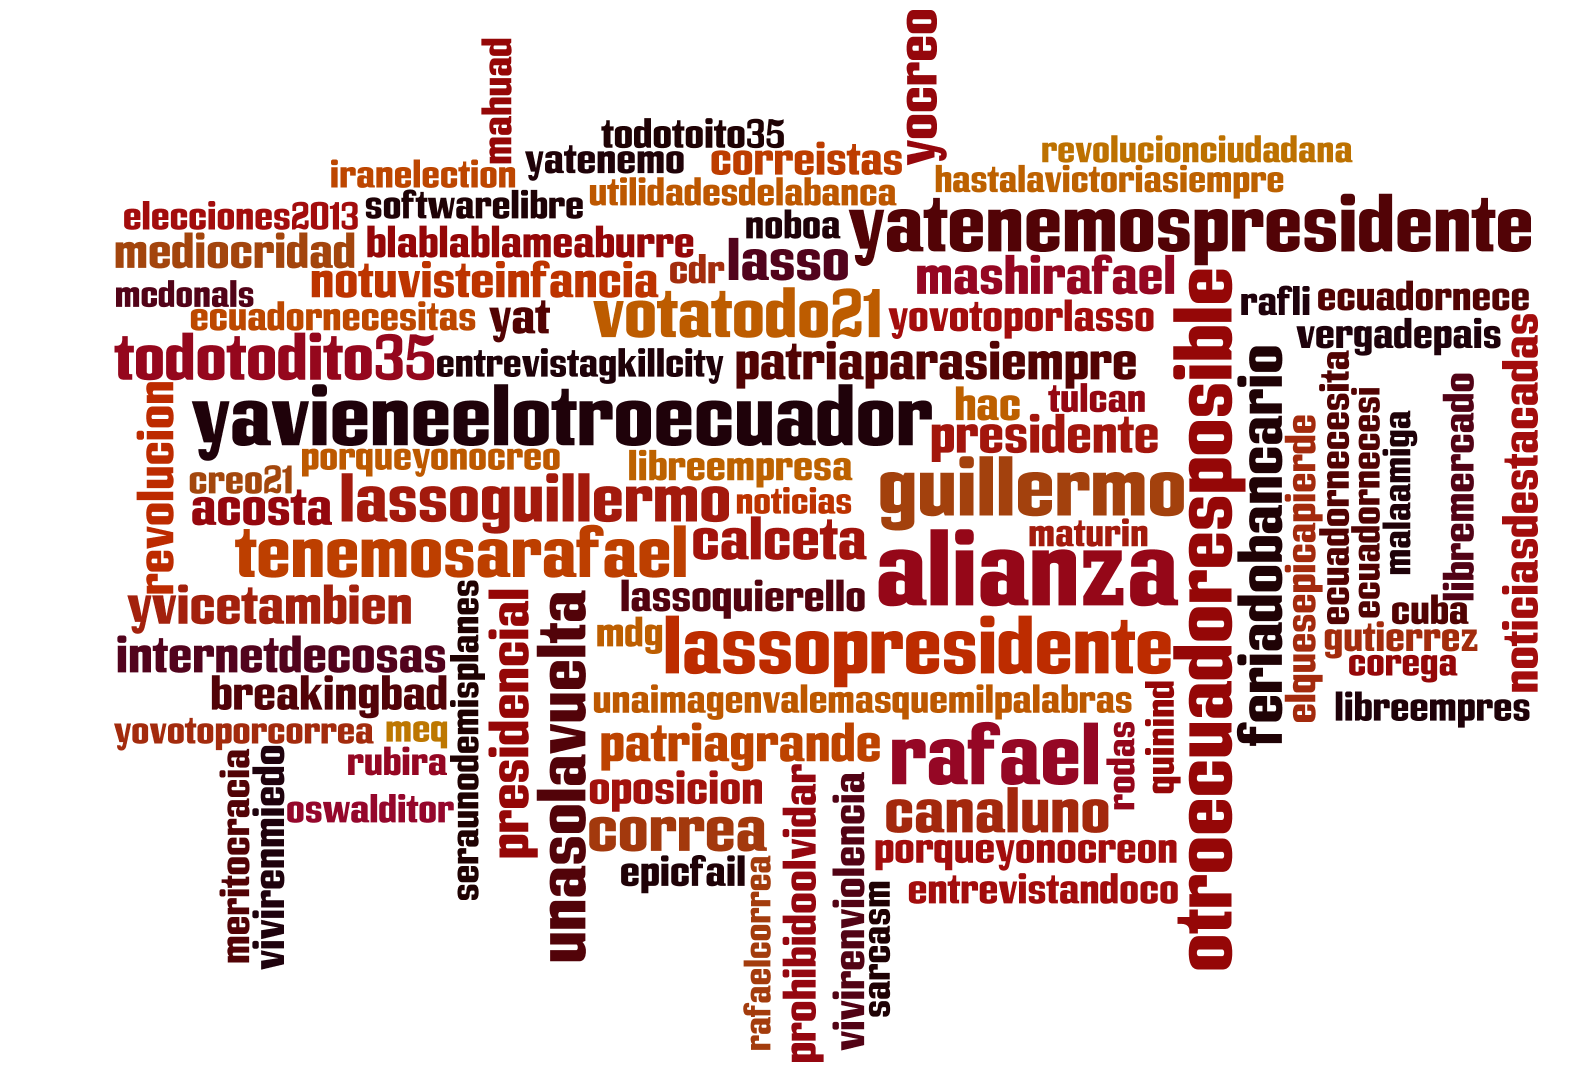
\includegraphics[width=0.5\textwidth, height=0.17\textheight]{support_files/ecuadorWordCloud.png}
		\label{fig:ecuadorwordCloud}
	}
	\caption{Vocabulary of hashtags identified for different elections} 
	\label{fig:countrywordCloud}
\end{figure*}
\noindent
{\bf Chile:}
Figure~\ref{fig:bacheletwordCloud} shows the hashtags identified for Michelle Bachelet who won the Chilean Presidential elections that was decided over two rounds.
The first round was conducted on the 24th of November, 2013 and the 2nd round was conducted on December 15, 2013. 
The query expansion pipeline for Bachelet's group in both these elections were initialized only with three seed words: {\it Bachelet, CommandoMichelle and PS}. 
The first name of the candidate was not used as it introduced a lot of noise because ``Michelle" is a very common name.
The first figure shows the hashtags identified for Bachelet during the first round and the second figure for the second round. 
It can be seen that there is a lot of overlap in the vocabulary which is the expected outcome. 
Similarly there were a lot of common hashtags between the two rounds of election for the other candidate, Evelyn Matthei, too.
%Figure~\ref{fig:countrywordCloud} shows the hashtags identified for the elections from Mexico, Paraguay, Honduras and Ecuador. 
It can be noticed that the vocabulary for the Honduran and Ecuadorean  elections are quite noisy. 
This is primarily because Twitter is not as popular in these two countries as in Venezuela or Chile and therefore the number of tweets
used for the inference was significantly lesser.
This in turn affects the quality of the PSL inference.

\TODO{}{Add analysis about latest presidential election in Colombia}

\TODO{}{Add analysis about latest presidential election in Costa Rica }

\TODO{}{Add analysis about latest presidential election in Panama}

\begin{comment}
\begin{table*}
        \centering
        \begin{tabular}{|l|r|}
        \hline
        Feature & Coefficient Value\\
        \hline
        \textrm{SoPU} & 0.4622\\
        \textrm{SoNU} & -0.443\\
        \textrm{SoPM} &  0.1158\\
        \textrm{SoNM} &  -0.065\\
        \textrm{SoS} & 0.156\\
        \textrm{Incumbency} & 0.0\\
        \hline
        \end{tabular}
        \caption{Regression coefficients learned for features; \textrm{SoPU}:Share of positive users;\textrm{SoNU}:Share of negative users;\textrm{SoPM}:Share of positive mentions;\textrm{SoNM}:Share of negative mentions;\textrm{Sos}:Share of sentiment;\textrm{Incumbency}:Binary variable for incumbency}
        \label{table:coeff}
\end{table*}
\end{comment}
%!TEX root = ../election_besc14.tex


\section{Experimental Results}
Our experimental results address the following questions:
\begin{itemize}
\item How adept is our PSL-based dynamic query expansion algorithm at extracting relevant hashtags/keywords over the course
of an election season?
\item How does the performance of forecasting algorithms improve using our expanded vocabularies?
\end{itemize}
We answer each of these questions next.

\subsection{Election vocabularies inferred}

\begin{figure}[Ht]
	\centering
	%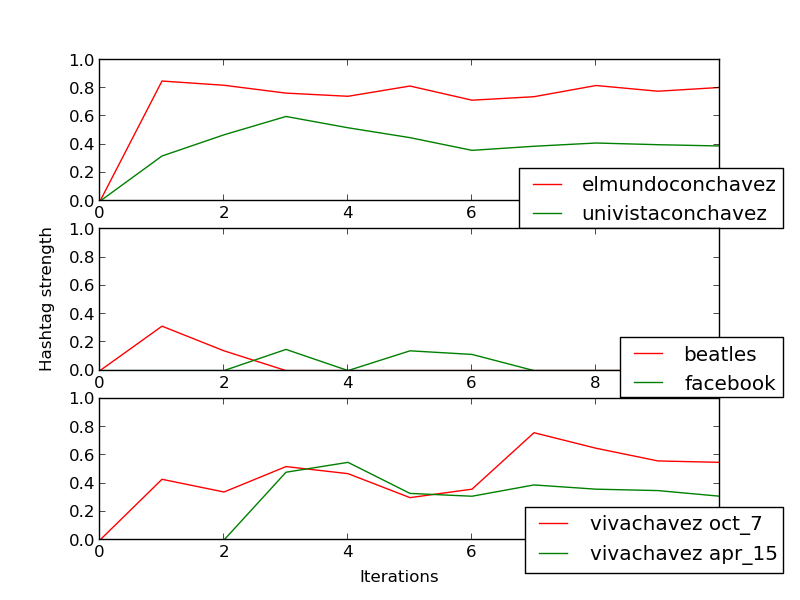
\includegraphics[scale=0.40]{support_files/hashTagTimeSeries.png}\\
	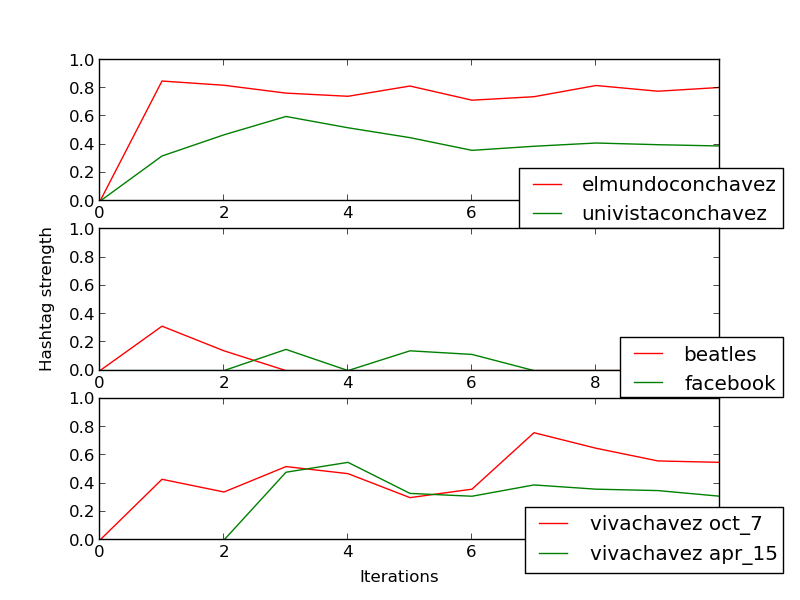
\includegraphics[height=0.2\textheight, width=0.45\textwidth]{support_files/hashTagTimeSeries.png}
	\caption{Evolution of different hashtags identified for Hugo Ch\'{a}vez in Venezuela 2012 presidential election}
	\label{fig:timeSeries}
\end{figure}

\begin{figure*}
	\centering
	\subfloat[Day 0]
	{
		
\includegraphics[width=0.5\textwidth, height=0.17\textheight]{support_files/caprilesWordCloud1.png}
		\label{fig:wordCloud1}
	} 
	\subfloat[Day 6]
	{
		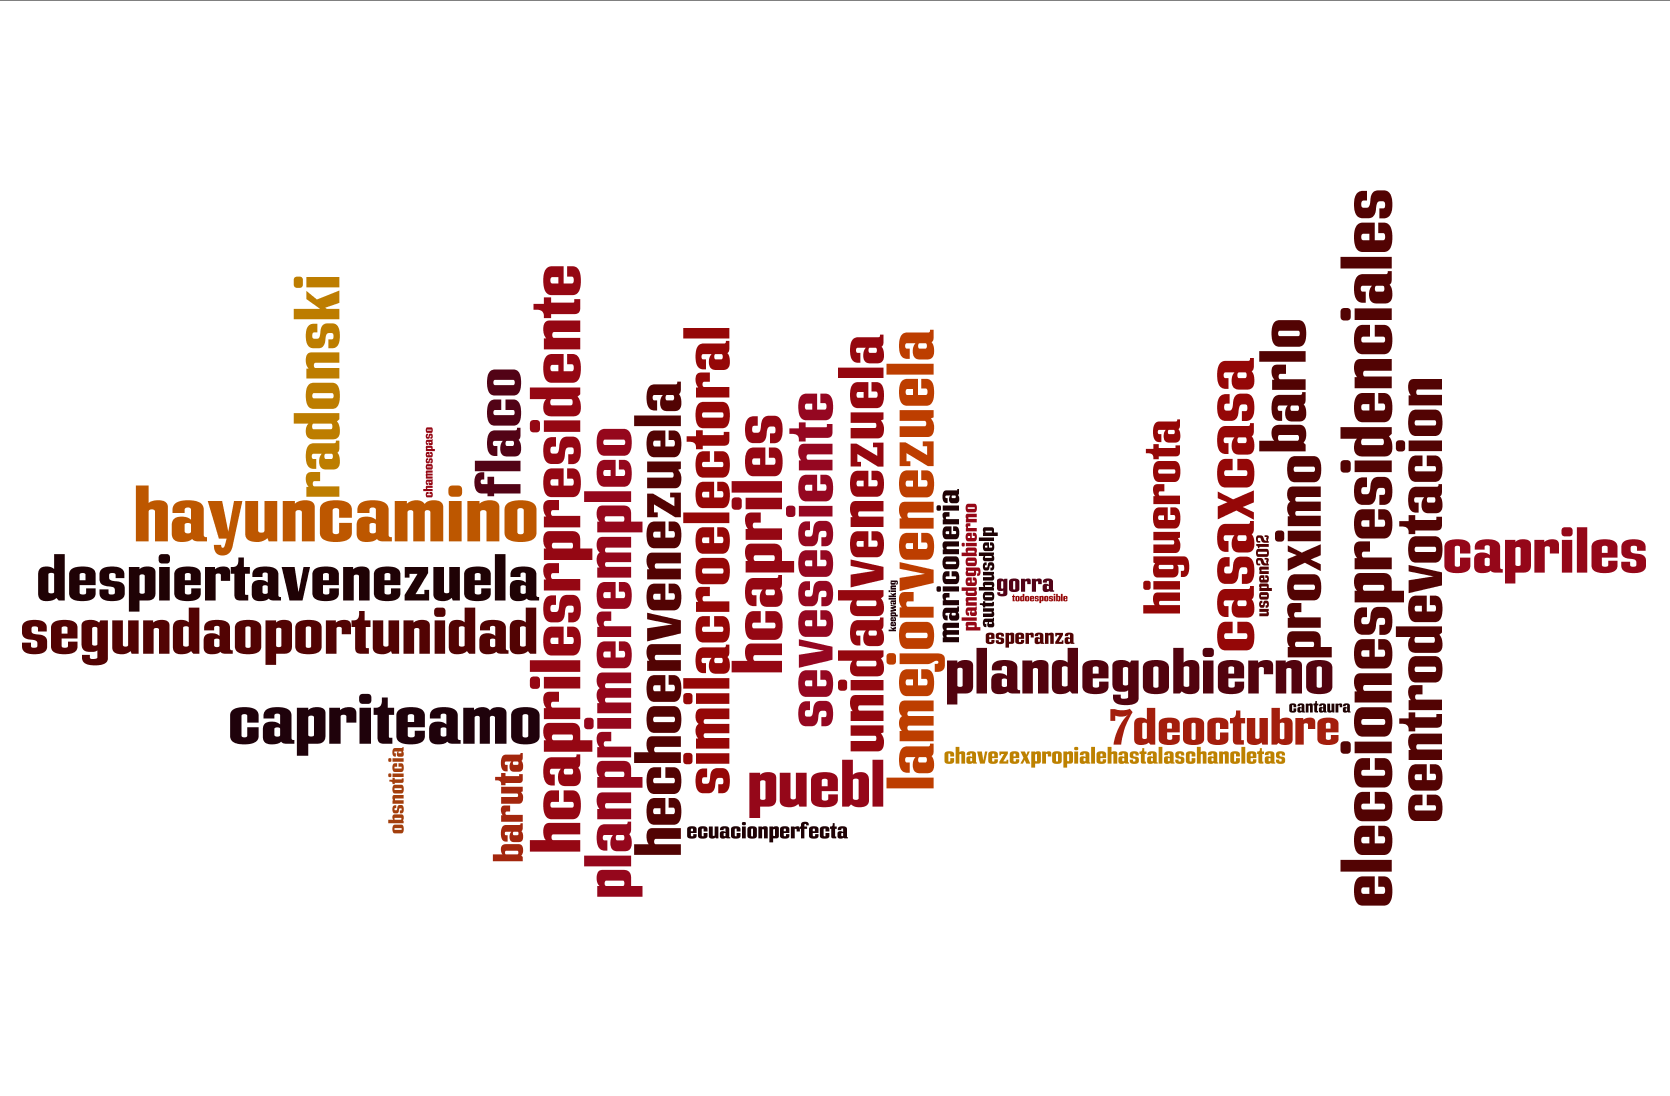
\includegraphics[width=0.5\textwidth, height=0.17\textheight]{support_files/caprilesWordCloud2.png}
		\label{fig:wordCloud2}
	} \\
	\noindent 
	\subfloat[Day 15]
	{
		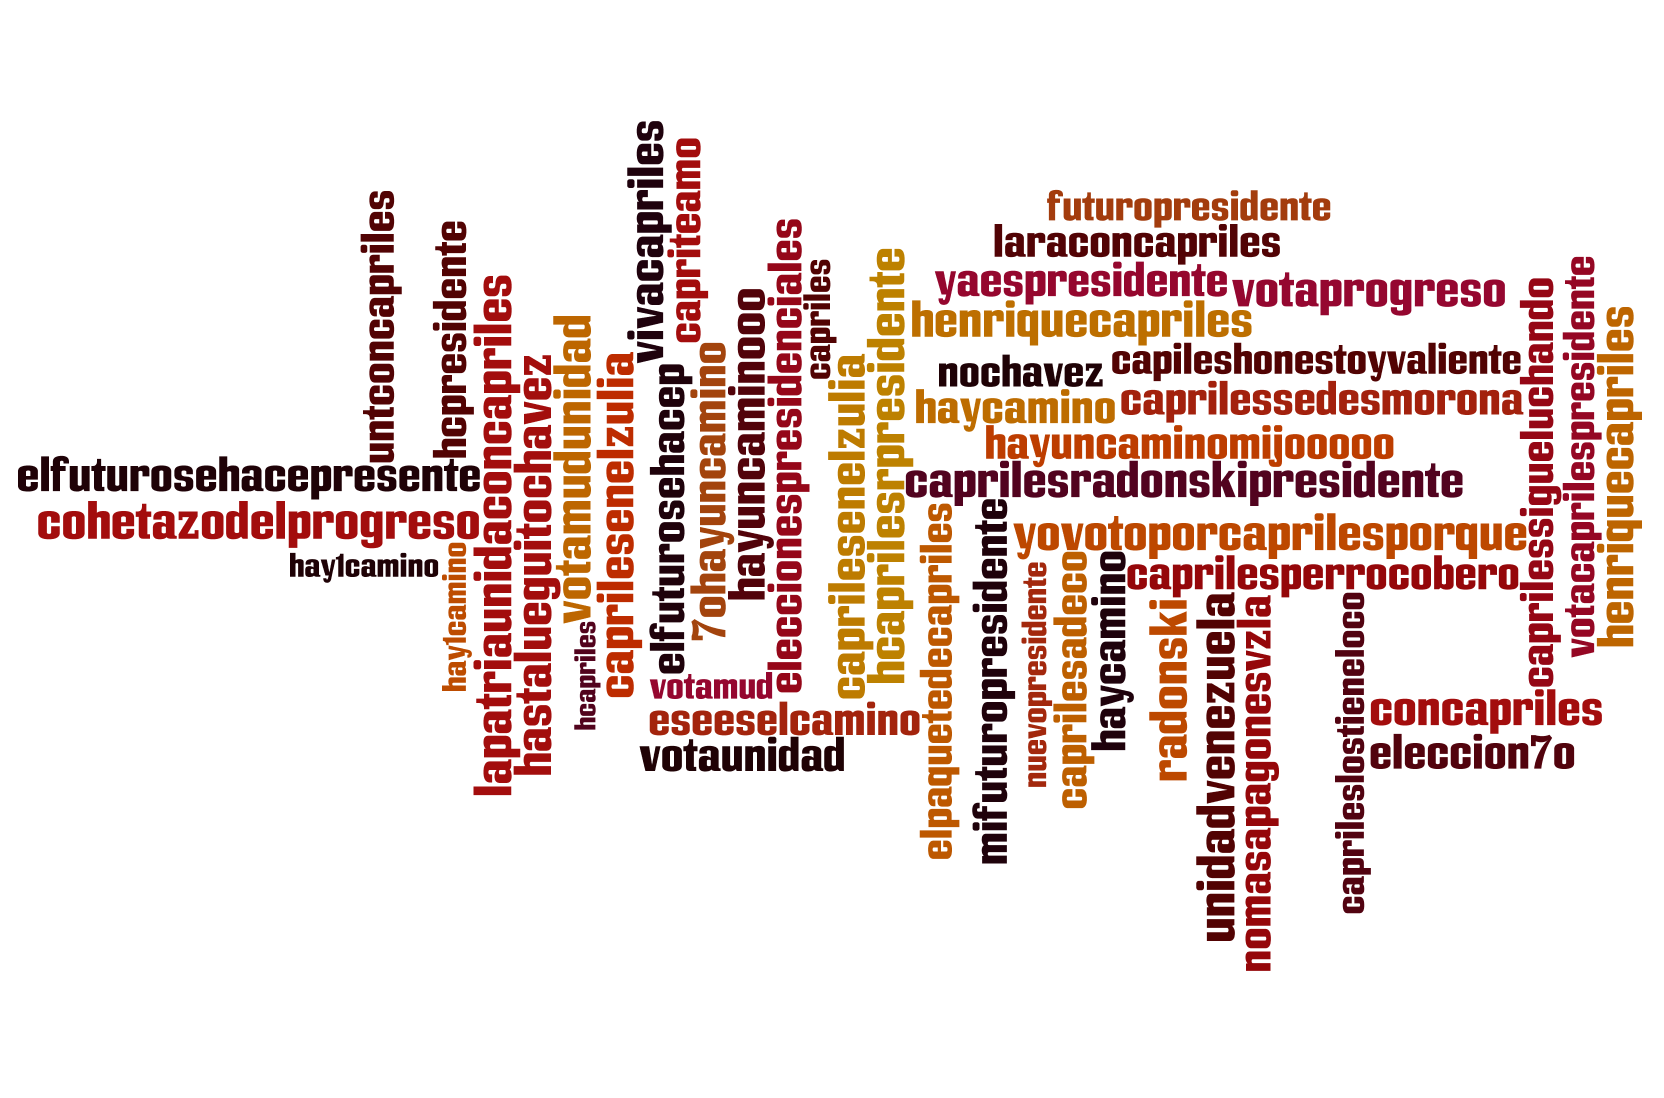
\includegraphics[width=0.5\textwidth, height=0.17\textheight]{support_files/caprilesWordCloud3.png}
		\label{fig:wordCloud3}
	}
	\subfloat[Day 30]
	{
		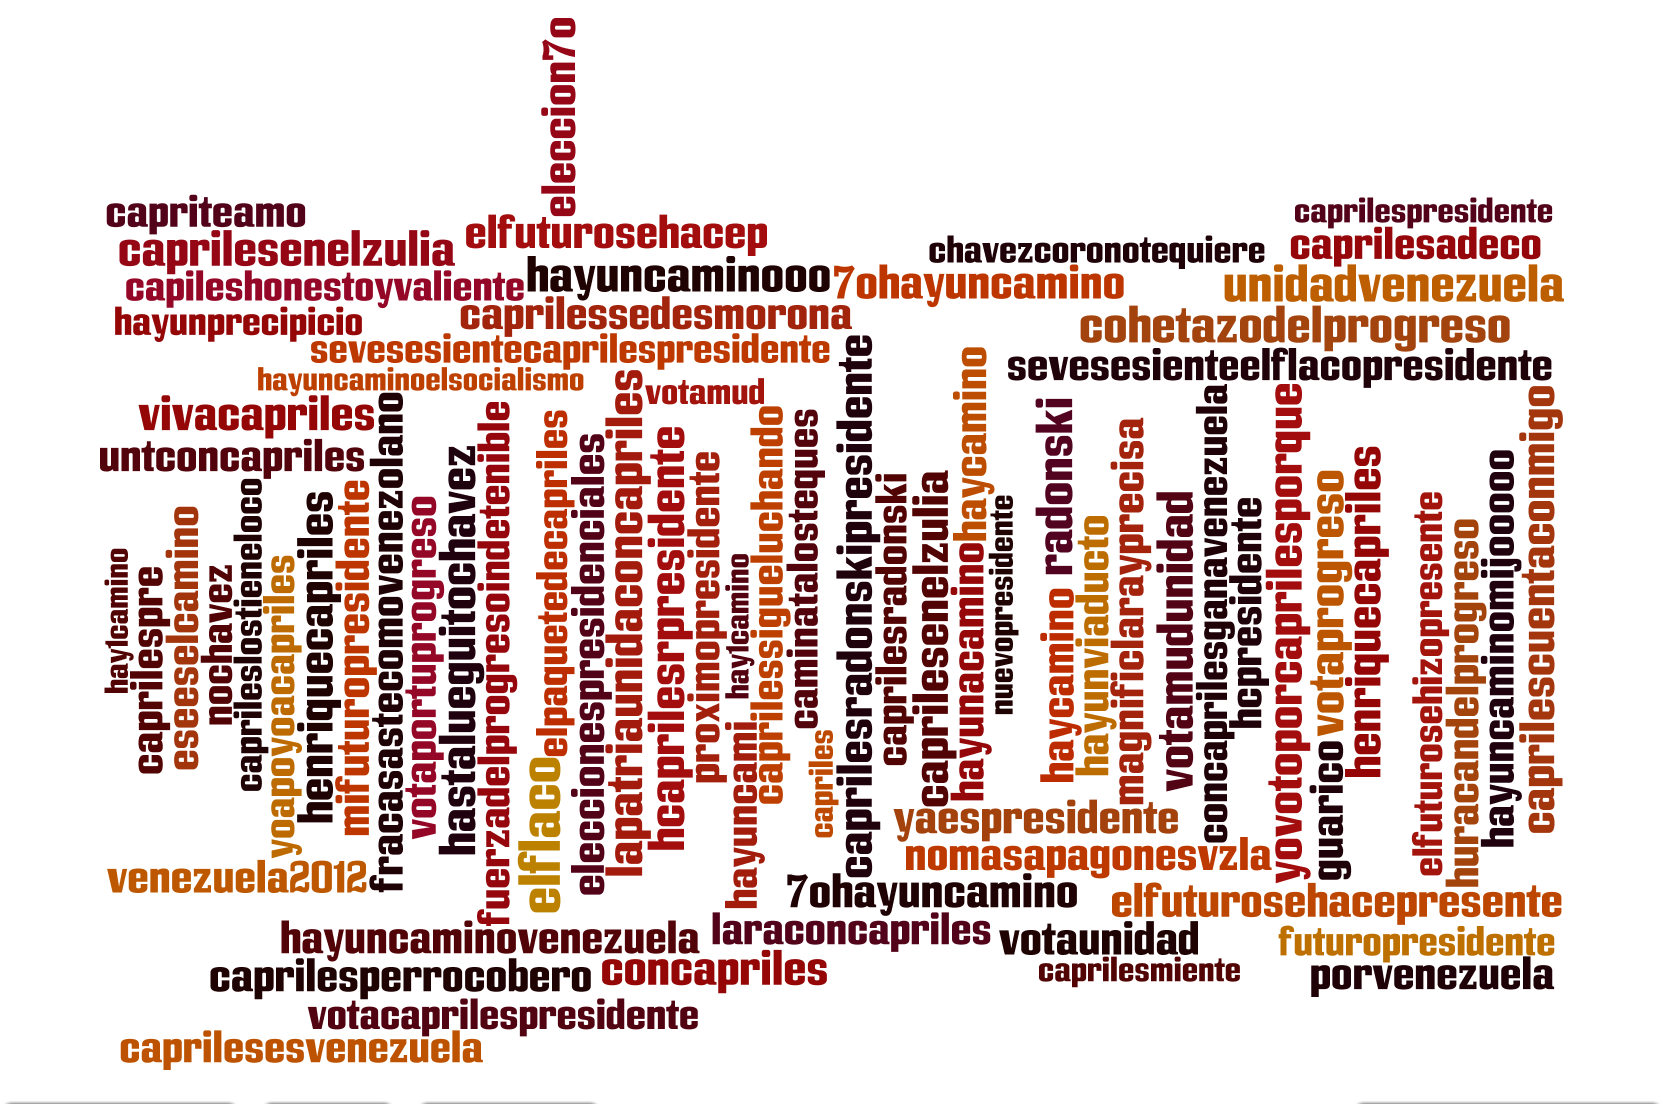
\includegraphics[width=0.5\textwidth, height=0.17\textheight]{support_files/caprilesWordCloud4.png}
		\label{fig:wordCloud4}
	}
	\caption{Evolution of hashtags for Henrique Capriles in 2013 Venezuela presidential election} 
	\label{fig:wordCloud}
\end{figure*}

\noindent
{\bf Venezuela:} 
Figure~\ref{fig:wordCloud} shows how the hashtags for Henrique Capriles evolved during the month leading up to the election.
Initially in Figure~\ref{fig:wordCloud1} the system begins with only a few hand picked hashtags that constitute the seed vocabulary. 
After a few iterations Figure~\ref{fig:wordCloud2} shows how the vocabulary has grown.
However, not all the words identified until now remain in the final vocabulary as the system drops certain words in successive iterations.
At the same time it is also noticed that hashtags like \emph{``capriles"} and \emph{``hayuncamino"} which are very strongly associated with Capriles consistently remain as the top ranked hashtags even after ten iterations (Figure~\ref{fig:wordCloud4}). 
It is also interesting to note that the algorithm identified hashtags like \emph{``nochavez"} (Figure~\ref{fig:wordCloud3}) and attributed it rightly to Hugo Ch\'{a}vez's primary contender, i.e., Capriles. 

In Figure~\ref{fig:timeSeries}, the first plot elucidates how hashtags like \emph{``elmnduconchavez"} and 
\emph{``univistaconchavez"} remain highly associated with Hugo Ch\'{a}vez for the October 7th Presidential election. 
These hashtags remain indicative of a user's affiliation throughout the month leading up to the election.
Meanwhile hashtags such as \emph{``beatles''} and \emph{``facebook''} (in second plot) show spikes in their time series primarily because users affiliated with Ch\'{a}vez used them during that time window. 
But as the iterative process continues, the system drops these non-informative words.
The third plot presents another interesting observation.
Hugo Ch\'{a}vez who had won the election on October 7, 2012 was diagnosed with cancer and passed away
before being sworn in as the President.
This triggered a re-election on April 15, 2013 where Nicolas Maduro, who had assumed the role of acting president then, competed 
against Henrique Capriles in the Presidential race.
The hashtag \emph{``vivachavez"} is part of both the elections, despite the 
fact that Hugo Ch\'{a}vez did not compete in the second election.
It is picked up as a phrase commonly used by supporters of Nicholas Maduro whose election campaign was strategized around the death of Hugo Ch\'{a}vez to garner sympathy and mobilize support.
Similarly variations of the hashtags \emph{``hayuncamino"} and \emph{``unidadvenuzela"} were returned 
for Henrique Capriles for both these elections.
The tag MUD is for \emph{``Mesa de la Unidad Democratica”} (Democratic Unity Roundtable) that was the organization created for the opposition to Ch\'{a}vez. 
The vocabulary grows to include other terms associated to the campaign, as the official slogan for the opposition \emph{``hayuncamino”} (there is a road). 
Others relate to programs that Capriles wanted to implement, such as \emph{``planprimerempleo”} (First Job Program). 

\noindent	
{\bf Mexico:} A general election in Mexico took place on July 1st, 2012.
The two front runners where Enrique Pe\'{n}a Nieto (EPN) and Andres Manuel L\'{o}pez Obrador (AMLO).
The tags (Figure~\ref{fig:mexicowordCloud}) show the contest between these two candidates, the first belonging to the \emph{“Partido Institucional Revolucionario”} (PRI). 
Among the tags we can also find reference to the \emph{“yosoy132”} student movement that became a key player during the election. 
%We have against AMLO some as “niunvotoalpeje” (no one vote for AMLO) or against EPN “soyantipri” (I am against PRI).
We also see \emph{“niunvotoalpeje”} (no one vote for AMLO) and \emph{“soyantipri”} (I am against PRI) which are attributed against AMLO and EPN respectively.

\noindent
{\bf Paraguay:}
Figure~\ref{fig:paraguaywordCloud} details the election between Horacio Cartes from the Partido Colorado and Efrain Alegre from Alianza Paraguay. 
The incumbent president belonged to Partido Colorado and we can see some tags talking about a protest vote: \emph{“votocastigoya”} (protest vote now). 
Also references from their campaign to each candidate as \emph{“yovotoporefrain”} (I vote for efrain) or \emph{“todosconcartesavanzapais”} (everyone with cartes, the country goes forward) are seen.

\noindent
{\bf Honduras:}
In November 2013 Honduras had a general election to choose President, Congress and local officials. 
The wife of former President Zelaya, Xiomara Castro, contended against Juan Orlando Hernandez from the incumbent Partido Nacional. 
Both candidates showed similar numbers in the polls before the election. 
We can find tags that either support Xiomara, like \emph{“xiomarapresidenta”} (Xiomara President), \emph{“hondurastienepresidenta”} (Honduras has a female president) or against her, \emph{“noaxiomara”} (no to Xiomara) in Figure~\ref{fig:honduraswordCloud}.

\noindent
{\bf Ecuador:}
Ecuador had a first round for the presidential election on February 17, 2013 where Rafael Correa obtained more than 50\% of the votes needed to avoid a second round. 
The tags (Fig.~\ref{fig:ecuadorwordCloud}) include support phrases such as \emph{“yatenemospresidente”} (we have elected president) or \emph{“tenemosarafael”} (we have Rafael). 
There are some references to other candidates such as \emph{“lassopresidente”} (candidate Lasso president).

\noindent
{\bf Colombia:}
The hashtags identified for Juan Manuel Santos who won the Colombian Presidential elections in the second round,
June 15 (first round May 25). The query expansion pipeline for these elections were initialized only with the main two candidates names: Santos, Manuel and Zuluaga, Ivan. We get some campain related slogans such as \emph{``enmigobiernoprometo''} (If I govern, I promise I will). Interestingly, these kind of hashtags are often used with a sarcastic tone.

\noindent
{\bf Panama:}
Panama's presidential election was held on May 4, with Juan Carlos Varela the winner. Seeding the query expansion pipeline were the last names of the candidates(Arias, Varela and Navarro) plus the initials of their parties(CD, PP and PRD respectively), with the addition of Arias' first name \emph{``Domingo''} to distinguish him from a former president, Oscar Arias. From the phrase \emph{``caminoalavictoria''} (road to victory), it indicates belief and faith that the candidate will win.

\begin{figure}
	\centering
	\subfloat[Nov 24]
	{
		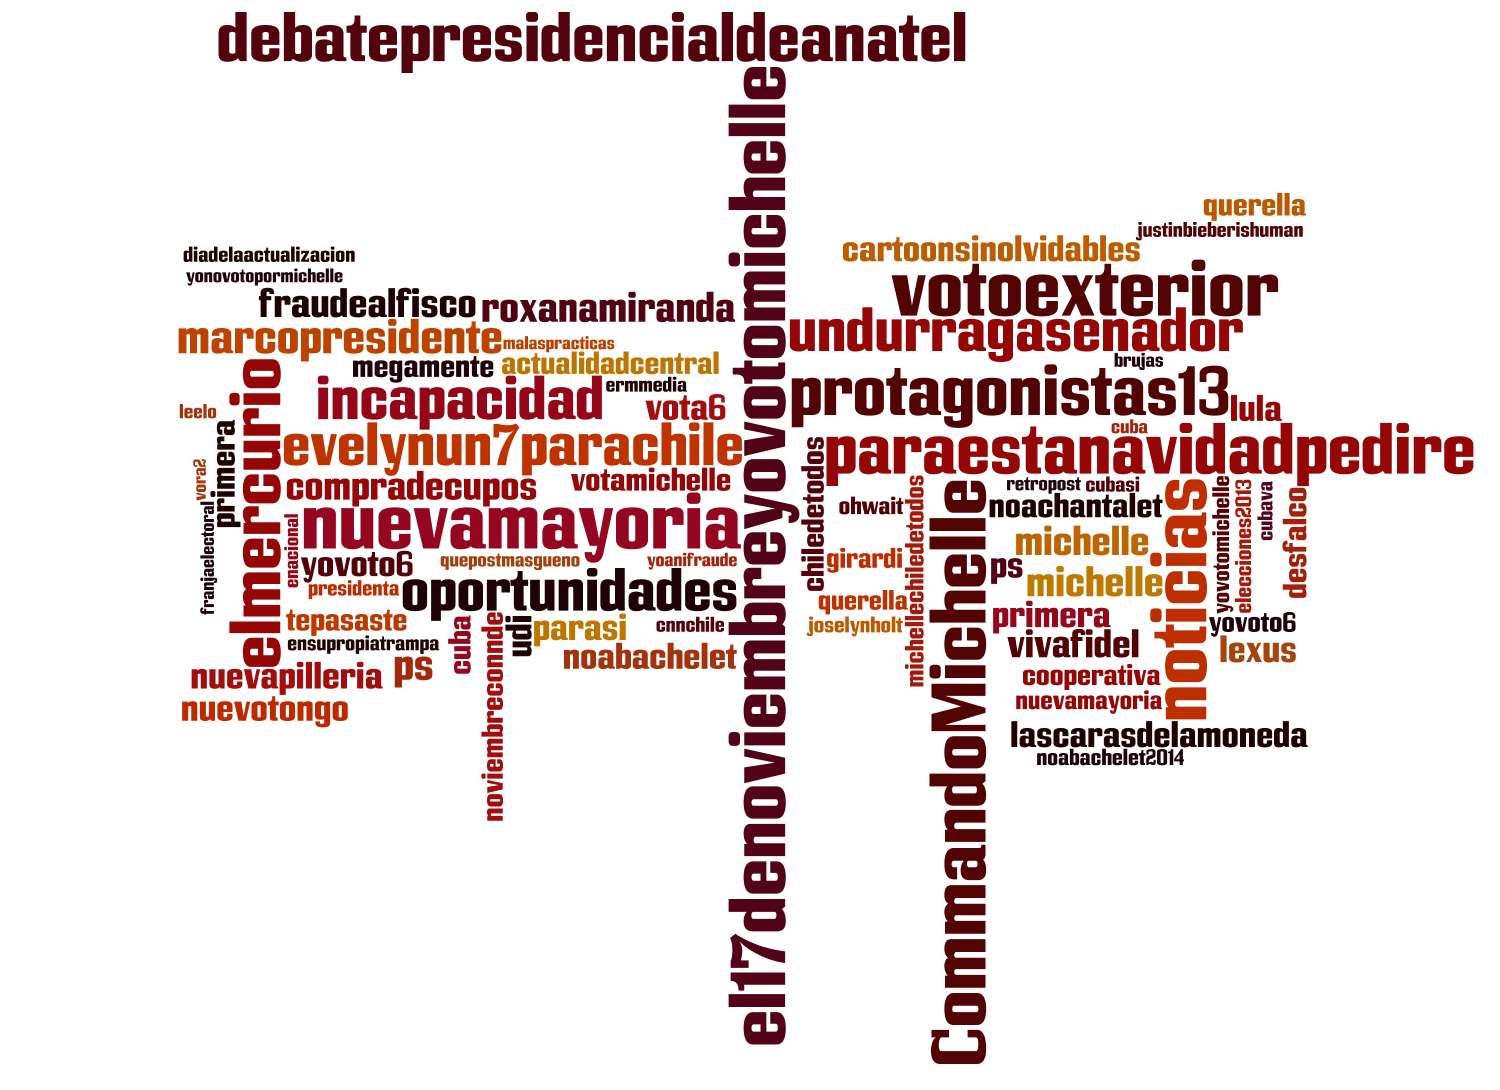
\includegraphics[width=0.22\textwidth, height=0.145\textheight]{support_files/bacheletWordCloud1.png}
		\label{fig:bacheletwordCloud1}
	} 
	\subfloat[Dec 15]
	{
		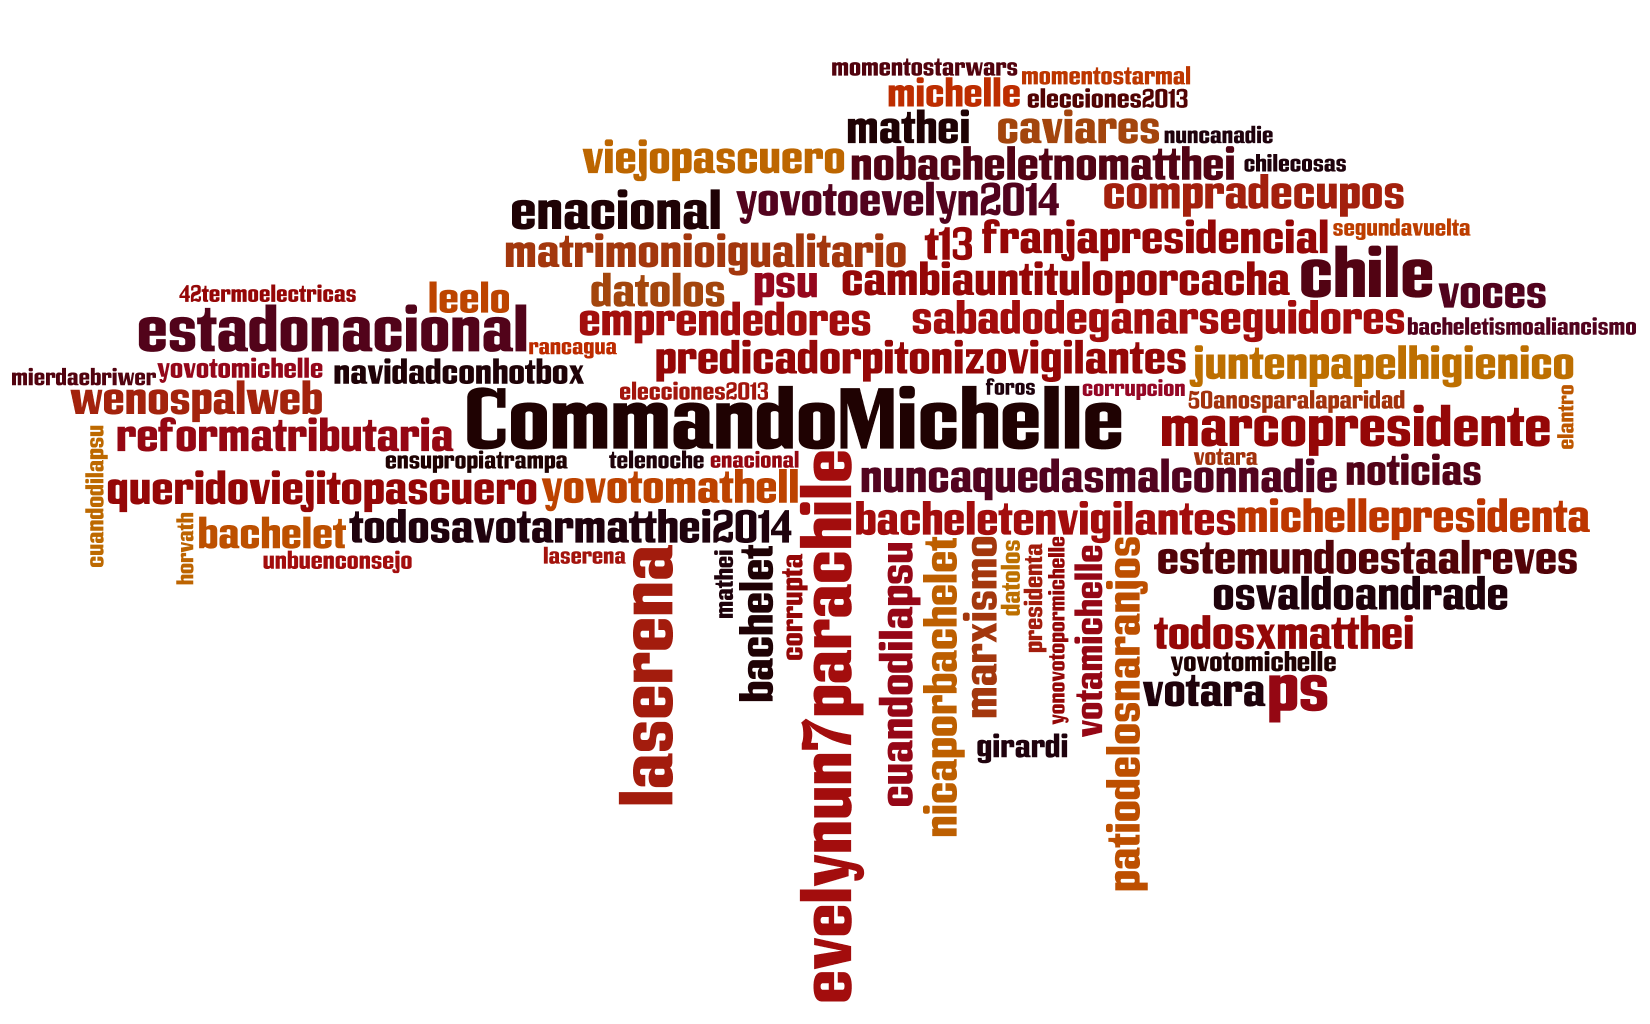
\includegraphics[width=0.22\textwidth, height=0.145\textheight]{support_files/bacheletWordCloud2.png}
		\label{fig:bacheletwordCloud2}
	}
	\caption{Hashtags identified for Michelle Bachelet in 2013 Chilean presidential election} 
	\label{fig:bacheletwordCloud}
\end{figure}

\noindent
{\bf Chile:}
Figure~\ref{fig:bacheletwordCloud} shows the hashtags identified for Michelle Bachelet, who won the Chilean Presidential elections that was decided over two rounds.
The first round was conducted on November 24, 2013 and the 2nd round was conducted on December 15, 2013. 
The query expansion pipelines for Bachelet's group in both these elections were initialized only with three seed words: {\emph{``Bachelet'', ``CommandoMichelle''} and \emph{``PS''}}. 
The first name of the candidate was not used as it introduced noise---\emph{``Michelle"} is a very common name.
The first figure shows the hashtags identified for Bachelet during the first round and the second figure for the second round. 
It can be seen that there is a lot of overlap in the vocabulary which is the expected outcome. 
Similarly there were a lot of common hashtags between the two rounds of election for the other candidate, Evelyn Matthei, too.
%Figure~\ref{fig:countrywordCloud} shows the hashtags identified for the elections from Mexico, Paraguay, Honduras and Ecuador. 
It can be noticed that the vocabulary for the Honduran and Ecuadorean  elections are quite noisy. 
This is primarily because Twitter is not as popular in these two countries as in Venezuela or Chile and therefore the number of tweets
used for the inference was significantly lesser.
This in turn affects the quality of the PSL inference.


\begin{figure}[t]
	\centering
	\subfloat[Mexico]
	{
		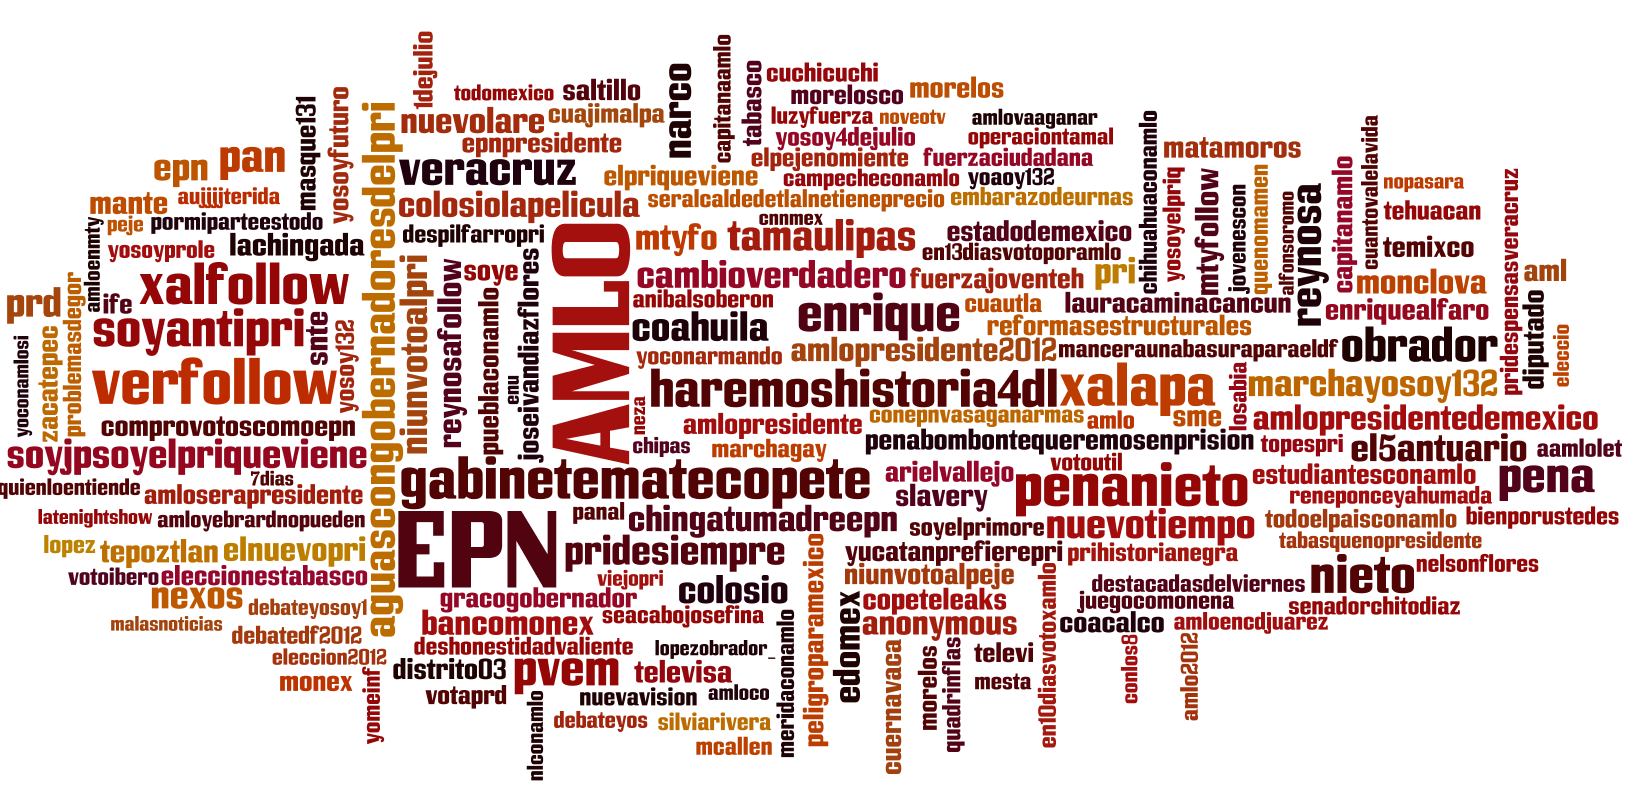
\includegraphics[width=0.22\textwidth, height=0.15\textheight]{support_files/mexicoWordCloud.png}
		\label{fig:mexicowordCloud}
	} 
	\subfloat[Paraguay]
	{
		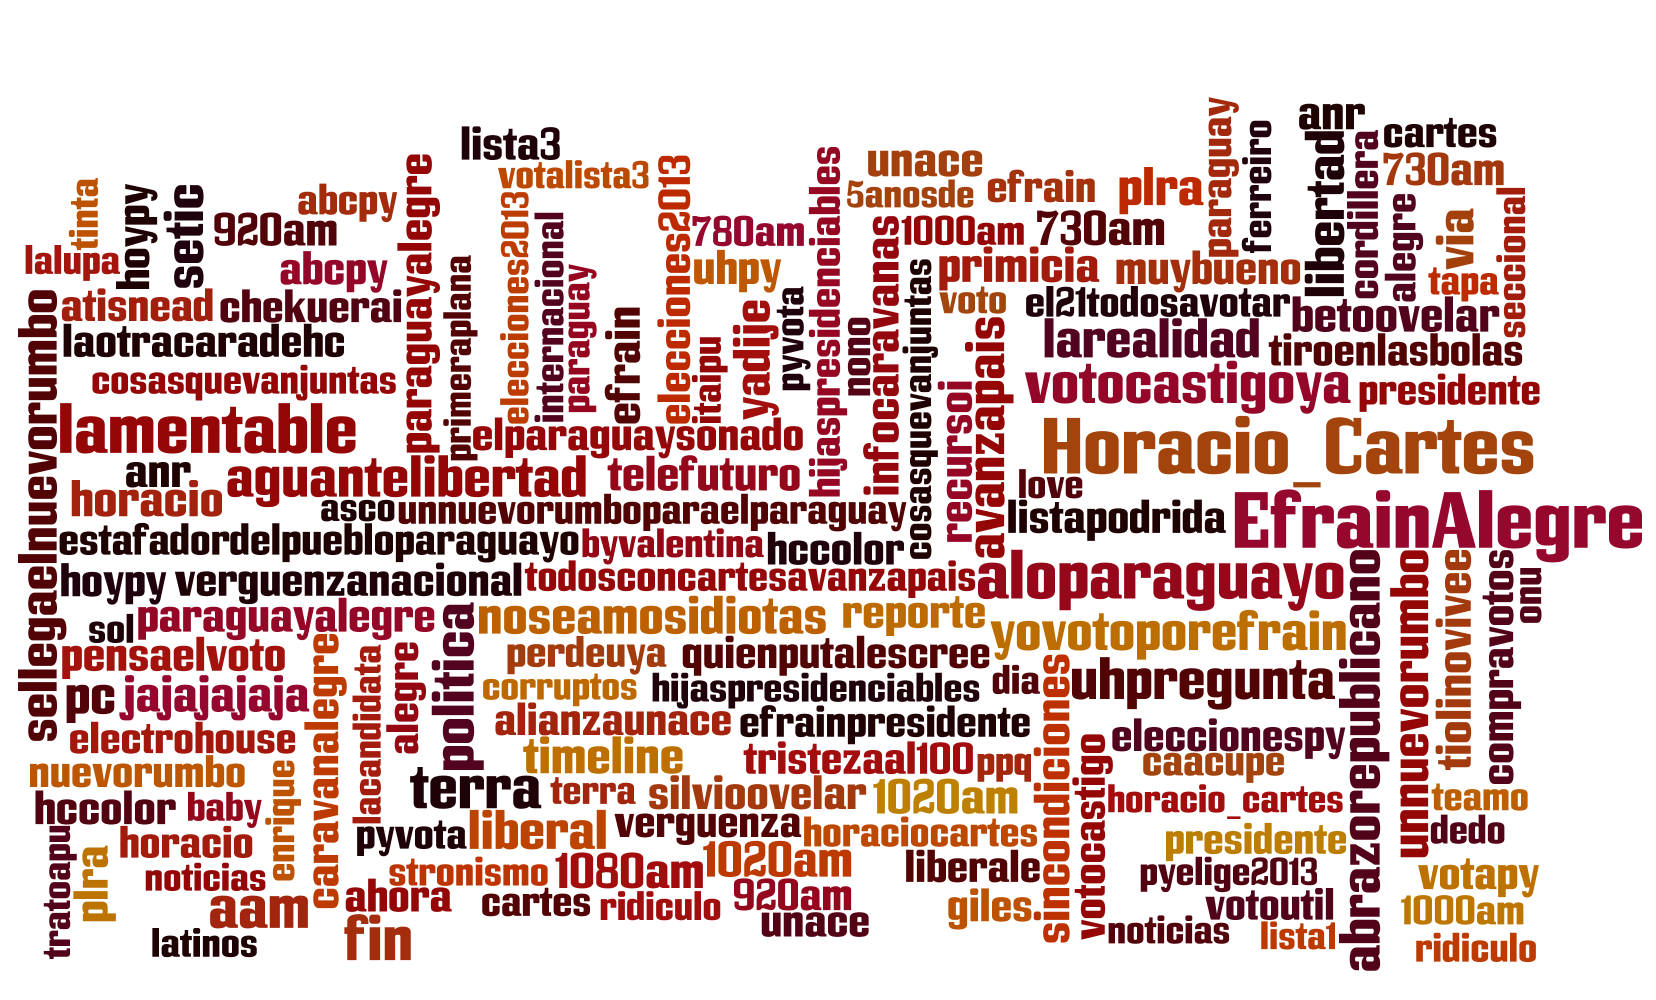
\includegraphics[width=0.22\textwidth, height=0.15\textheight]{support_files/paraguayWordCloud.png}
		\label{fig:paraguaywordCloud}
	} \\
	\noindent 
	\subfloat[Honduras]
	{
		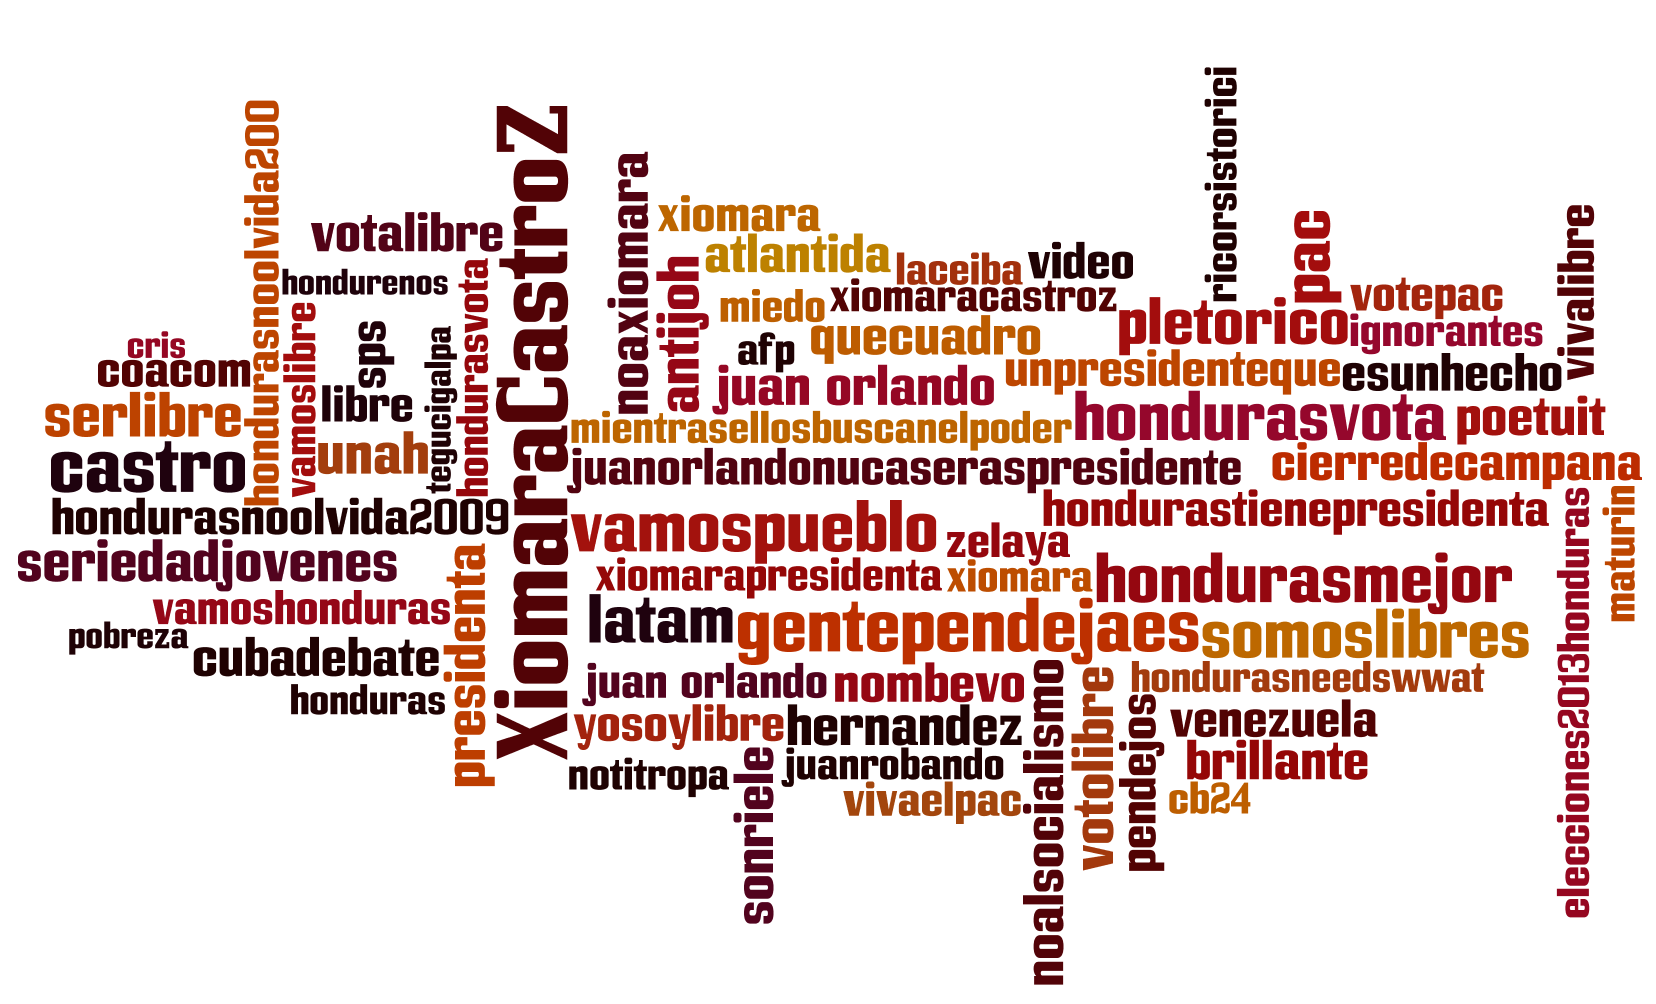
\includegraphics[width=0.22\textwidth, height=0.15\textheight]{support_files/hondurasWordCloud.png}
		\label{fig:honduraswordCloud}
	}
	\subfloat[Ecuador]
	{
		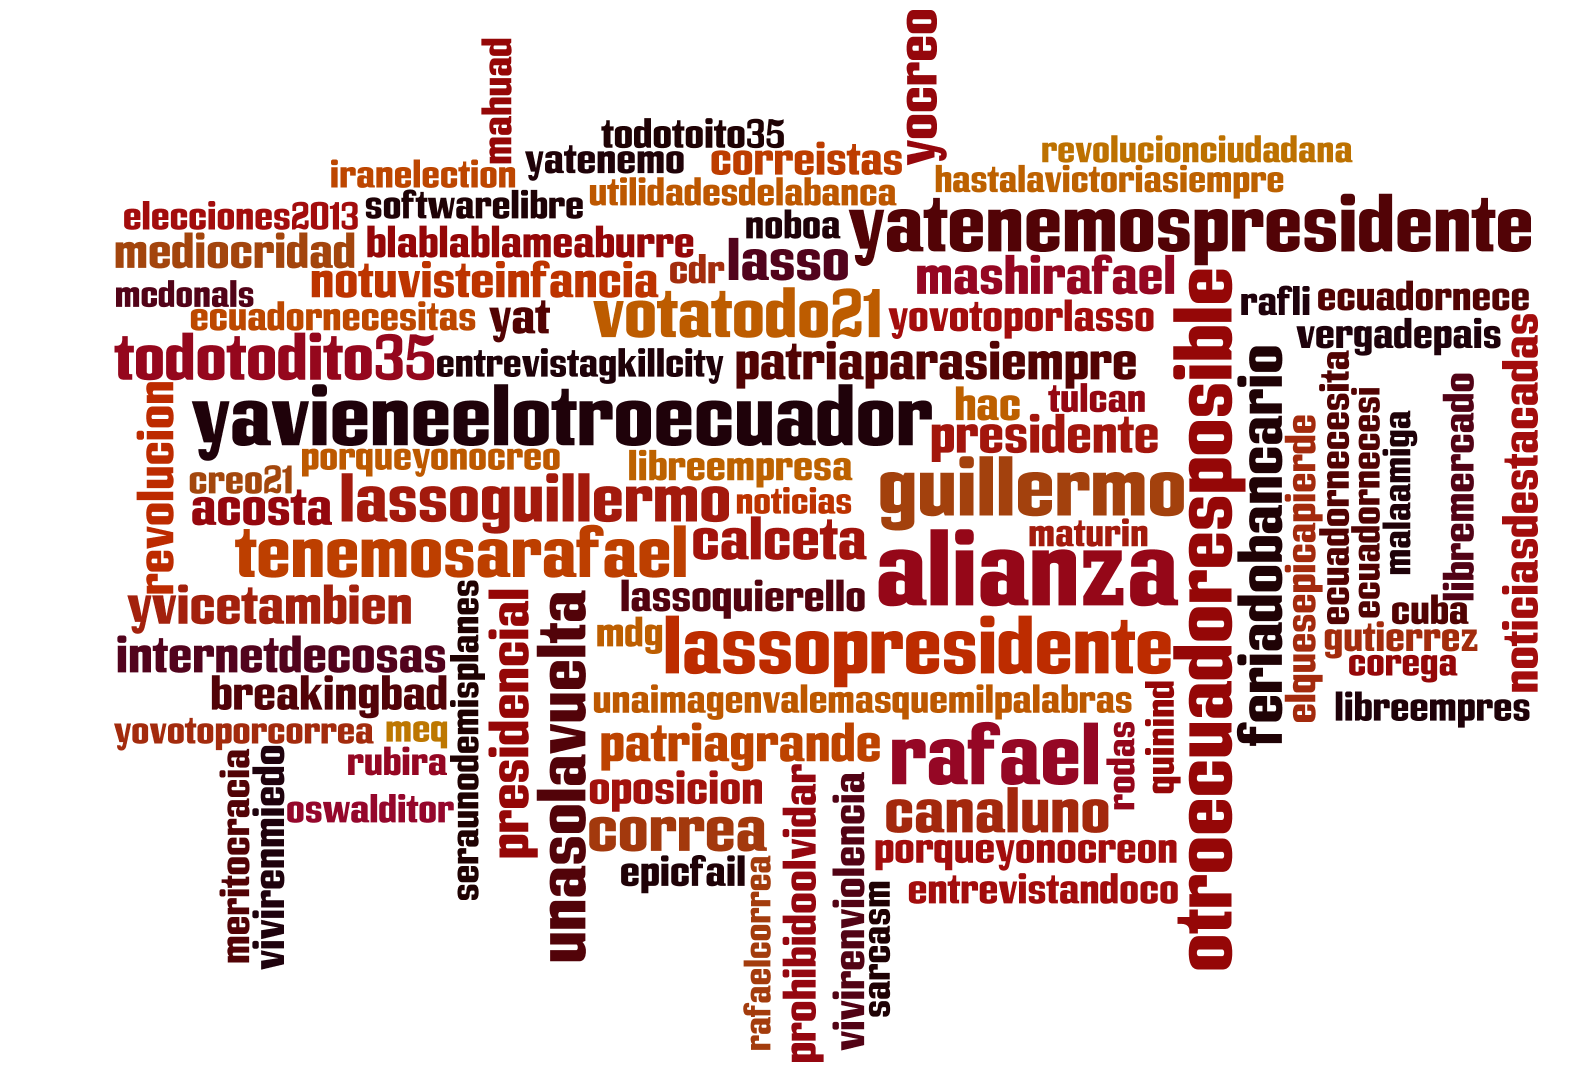
\includegraphics[width=0.22\textwidth, height=0.15\textheight]{support_files/ecuadorWordCloud.png}
		\label{fig:ecuadorwordCloud}
	}\\
	\noindent 
	\subfloat[Colombia]
	{
		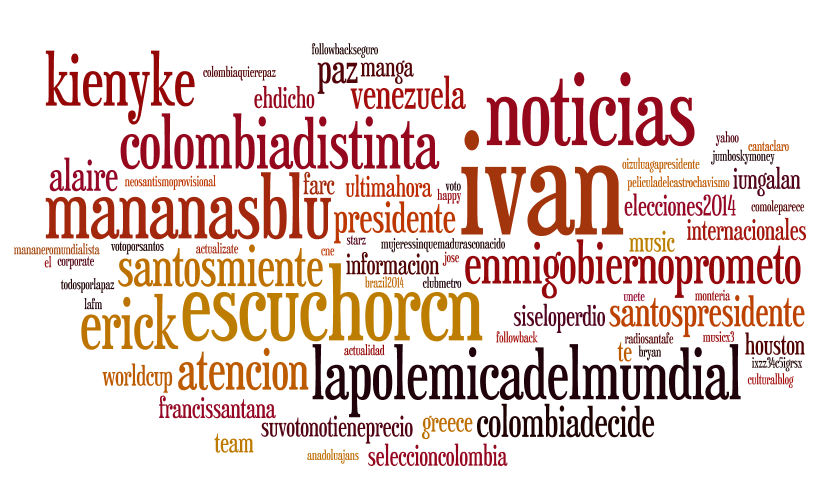
\includegraphics[width=0.22\textwidth, height=0.15\textheight]{support_files/colombia_cloud.png}
		\label{fig:colombiawordCloud}
	}
	\subfloat[Panama]
	{
		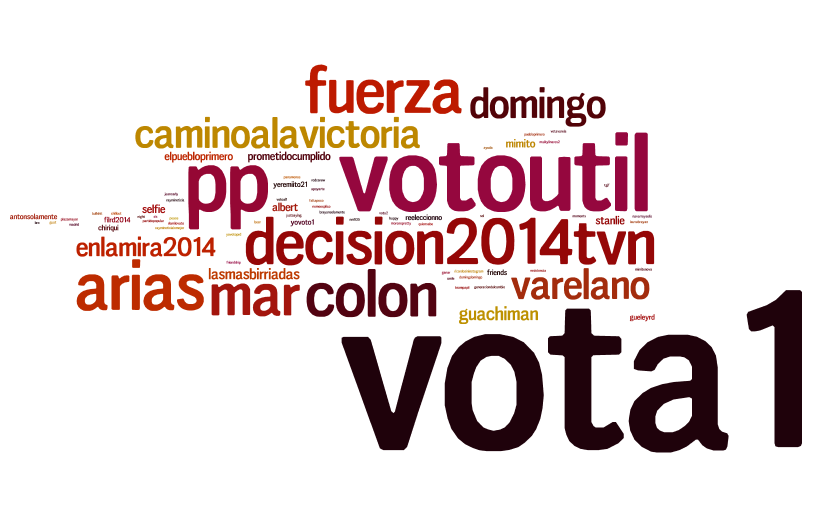
\includegraphics[width=0.22\textwidth, height=0.15\textheight]{support_files/panama_cloud.png}
		\label{fig:panamawordCloud}
	}
	\caption{Vocabulary of hashtags identified for different elections} 
	\label{fig:countrywordCloud}
\end{figure}
\noindent


\subsection{Election Prediction}
\begin{comment}

\begin{table*}[ht]
	\centering
	\begin{tabular}{| l |l| r | r |}
		\hline
		Election Type & Winner& Seed Words & PSL Expansion\\
		\hline
		2012 Mexico & Enrique Peña Nieto&  & True \\
		2012 Venezuela & Hugo Ch\'{a}vez& & True\\
		2013 Venezuela & Nicolás Maduro & & True\\
		2013 Chile first round & Michelle Bachelet & True& True\\
		2013 Chile second round & Michelle Bachelet  & True & True\\
		2013 Ecuador & Rafael Correa & True& True\\
		2013 Honduras & Juan Orlando Hernández  & False& \\
		2013 Paraguay & Horacio Cartes & True& True\\
		2014 Colombia first round & Óscar Iván Zuluaga & False& True\\
		2014 Colombia second round & Juan Manuel Santos & False& False\\
		2014 Panama & Juan Carlos Varela& False& True\\\hline
		Average Accuracy &    & \%& \%\\
		\hline
	\end{tabular}
	\caption{Track Record of Prediction Algorithms(Need to complete experiments on the missing countries)}
	\label{table:trackRecord2}
\end{table*}

\end{comment}
		
\begin{table*}[ht]
		\centering
		\begin{tabular}{| l | l | r | r | r | r | r | r |}
		\hline
		Election & Candidate & Actual Result & Seed Vocab. & Error & PSL Vocab. & Error \\
		\hline
		\multirow{2}{*}{Mexico\_Jul01} & Pe\~{n}a Nieto & 38.1 & 46.80 & 8.65 & 39.00 & \textbf{0.85} \\\cline{2-7}
											   & L\'{o}pez Obrador & 31.64 & 24.67 & 6.97 & 28.64 & \textbf{3.00} \\
		\hline
		\multirow{2}{*}{Venezuela\_Oct7} & Hugo Ch\'{a}vez & 55.07 & 49.89 & 5.18 & 55.89 & \textbf{0.82}\\\cline{2-7}
																& Henrique Capriles & 44.31 & 36.31 & 8.00 & 43.91 & \textbf{0.40} \\
		\hline
		\multirow{2}{*}{Ecuador\_Feb17} & Rafael Correa & 57.16 & 53.33 & 3.84 & 54.33 & \textbf{2.84} \\\cline{2-7}
												 & Guillermo Lasso & 22.68 & 12.27 & 10.41 & 12.75 & \textbf{9.93} \\
		\hline
		 \multirow{2}{*}{Venezuela\_Apr15} & Nicol\'{a}s Maduro & 50.61 & 51.45 & 0.84 & 50.58 & \textbf{0.03} \\\cline{2-7}
																	& Henrique Capriles & 49.12 & 35.96 & 13.16 & 38.11 & \textbf{11.01} \\
		\hline
		\multirow{2}{*}{Paraguay\_Apr21} & Horacio Cartes & 48.48 & 35.21 & 13.27 & 40.63 & \textbf{7.85} \\\cline{2-7}
												   & Efra\'{i}n Alegre & 39.05 & 31.33 & 7.72 & 34.44 & \textbf{4.62} \\
		\hline
		\multirow{2}{*}{Chile\_Nov17} & Michelle Bachelet & 46.70 & 38.91 & 7.79 & 41.80 & \textbf{4.91}\\\cline{2-7}
														  & Evelyn Matthei & 25.03 & 19.20 & 5.83 & 20.98 & \textbf{4.05} \\
		\hline 
		\multirow{2}{*}{Honduras\_Nov24} & Orlando Hern\'{a}ndez & 36.80 & 25.16 & 11.64 & 28.30 & \textbf{8.50} \\\cline{2-7}
												   & Xiomara Castro & 28.70 & 16.53 & 12.17 & 24.90 & \textbf{3.80} \\
		\hline
		\multirow{2}{*}{Chile\_Dec15} & Michelle Bachelet & 62.16 & 39.12 & 23.04 & 39.80 & \textbf{22.37}\\\cline{2-7}
															& Evelyn Matthei & 37.83 & 20.88 & 16.95 & 21.68 & \textbf{16.15} \\
		\hline
		\multirow{2}{*}{Panama\_May04} & Juan Carlos Varela & 39.07 &31.28  & 7.79 & 36.23  & \textbf{2.84}\\\cline{2-7}
																	& Jose Domingo Arias  & 31.40 & 35.02  & 3.62  & 33.67  & \textbf{2.27} \\
		\hline 											 
		\multirow{2}{*}{Colombia\_Jun15} & Juan Manuel Santos & 50.95 &48.85  & \textbf{2.1} & 45.75 & 5.2\\\cline{2-7}
																	& Oscar Ivan Zuluaga & 45.00 & 43.79 & \textbf{1.21} & 46.72  & 1.72 \\
		\hline
		\end{tabular}
		\caption{Reduction in prediction error for Regression Model. All values shown are percentages.}
		\label{table:trackRecord}
	\end{table*}	

We adapt one basic forecasting algorithm from current literature to evaluate the
performance of our expanded vocabularies. The model uses a regression fit to map from tweet features to opinion polls and thus forecast elections. We dub this model as the \emph{``regression model"} and this approach is adapted from \cite{bermingham2011using} and \cite{o2010tweets}.

{\bf Regression Model:}
In this model, in addition to tweets, we leverage any opinion polls available for the elections 
to make our predictions.
Like the earlier model we track the tweets that mention words/phrases
from the vocabulary defined for each candidate.
We then conduct a linear regression fit that uses the opinion polls as dependent variable and features generated from 
these tweets as independent variable.
We reason that by regressing from the Twitter features to the opinion polls the bias due to Twitter being a non-representative sample
can be mitigated.
We use a total of six features: Klout scores, number of unique users, total number of mentions, sentiment, and incumbency.
The Klout scores, unique users, and mentions are further categorized into positive and negative mentions.
We normalize each of these features across all candidates to obtain the relative share of the volume. 
When there is more than one polling house publishing an opinion poll (for the same date) we take the average of the polls. 

\noindent
{\bf Performance:}
The Regression Model was tested exhaustively on a total of 11 presidential elections from Latin America during 2012 and 2014. we run the prediction model in two different setting: only using the seeding words and using PSL query expansion.The tweets were purchased from DataSift, an infoveilence service that resells Twitter data. Then these tweets were geo-coded using a geo-location algorithm we developed to obtain tweets from the country of interest.
Only tweets from the locations pertaining to elections were used to make the predictions.
For example, for the Colombia 2014 presidential elections only tweets from Colombia were used.
Once the tweets were filtered by location the time series of Klout and sentiment scores were calculated by tracking the tweets for the mentions of candidate.

Table~\ref{table:trackRecord} shows the overall performance of the regression model under two settings. For each election, we predict the support rate for each candidate. The error rate is calculated as the difference between actual support rate and our prediction.
Although both of two settings have the same accuracy 0.9, but the overall error rate has been significantly inproved by applying PSL query expansion. 

\section{Discussion}
We have demonstrated a novel query expansion methodology using PSL and illustrated our method could correctly capture the evolving election related vocabularies during the election season.
We believe that the dynamic query expansion system is general and can be applied to a lot of domains such as election prediction, information retrieval.
In future work, we aim to more finely model information about electoral demographics and study
interactions both at the group and at the individual level. We also intend to use labeled data to learn
PSL programs (both structure and probabilities). Finally, we aim to use the framework presented
here as a platform to investigate theories of how social groups participate and influence elections.



\begin{comment}
\textbf{Acknowledgments}
This work is supported in part by the National Science Foundation under Grant No. 0937094 and the Intelligence Advanced Research Projects Activity (IARPA) via Department of Interior National Business Center (DoI/NBC) contract number D12PC00337. The U.S. Government is authorized to reproduce and distribute reprints for Governmental purposes notwithstanding any copyright annotation thereon. Disclaimer: The views and conclusions contained herein are those of the authors and should not be interpreted as necessarily representing the official policies or endorsements, either expressed or implied, of IARPA, DOI/NBA, or the U.S. Government.
\end{comment}

\bibliographystyle{IEEEtran}
\bibliography{references}

\begin{comment}
\begin{figure*}
	\centering
	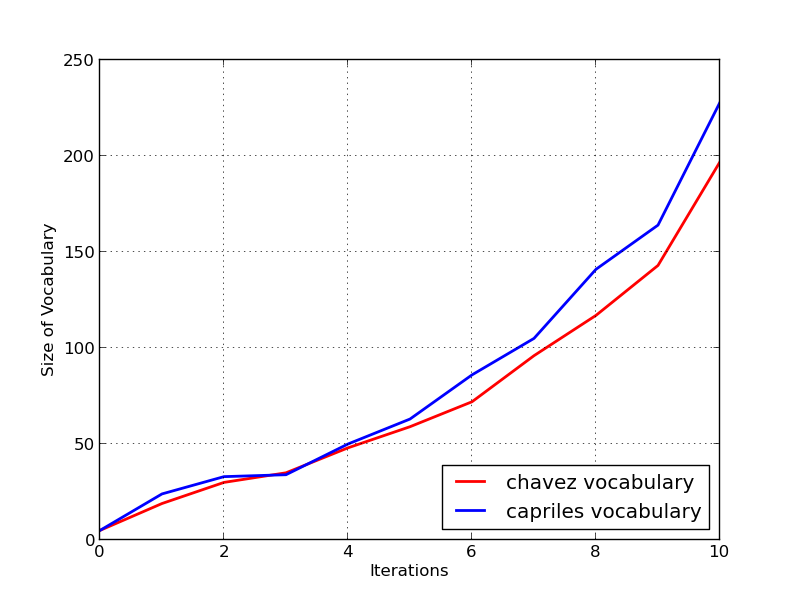
\includegraphics[height=0.3\textheight, width=0.80\textwidth]{support_files/WordGrowth.png}
	%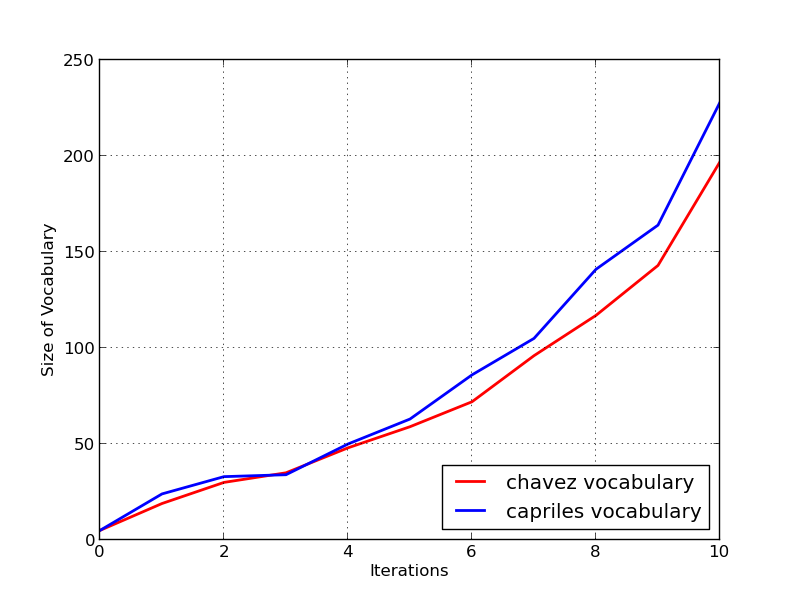
\includegraphics[scale=0.30]{support_files/WordGrowth.png}
	\caption{Vocabulary growth with each iteration.}
	\label{fig:wordgrowth}
\end{figure*}
\end{comment}


\end{document}


